% ============================================================================
%  EC486 Minor Project — FINAL REPORT
%  SiliconScribe: Execution-Grounded RTL Generation and Autonomous Diagnosis
%
%  Student : Kushal Pitaliya (23EC105)
%  Institute: CHARUSAT — CSPIT, V.T. Patel Dept. of ECE
%
%  Build: tectonic EC486_Final_Report.tex   (run from docs/)
% ============================================================================

\documentclass[11pt,a4paper]{article}

% ---------------------------------------------------------------- layout ----
\usepackage[a4paper,margin=2.15cm,top=2.15cm,bottom=2.15cm,headheight=14pt,headsep=13pt,footskip=17pt]{geometry}
\usepackage[T1]{fontenc}
\usepackage[utf8]{inputenc}
\usepackage{courier}
\renewcommand{\ttdefault}{cmtt}

% --------------------------------------------------------------- graphics ----
\usepackage{amsmath}
\usepackage{graphicx}
\graphicspath{{screenshots/}{docs/screenshots/}}
\usepackage{xcolor}
\usepackage{tikz}
\usetikzlibrary{arrows.meta,positioning,shapes.geometric,calc,fit}
\usepackage{listings}
\usepackage{float}

% ----------------------------------------------------------------- tables ----
\usepackage{booktabs}
\usepackage{array}
\usepackage{tabularx}
\usepackage{multirow}

% ------------------------------------------------------------- typography ----
\usepackage{microtype}
\usepackage{enumitem}
\setlist{nosep,leftmargin=*}
\usepackage{titlesec}
\usepackage{caption}
\captionsetup{font=small,labelfont={bf},justification=justified}
\usepackage{fancyhdr}
\usepackage{lastpage}
\usepackage{hyperref}
\hypersetup{hidelinks,pdftitle={SiliconScribe - EC486 Final Report},
            pdfauthor={Kushal Pitaliya (23EC105)}}
\usepackage{xurl}

\setlength{\emergencystretch}{1.5em}

% ----------------------------------------------------------- colour setup ---
\definecolor{ink}{RGB}{0,0,0}
\definecolor{inkdark}{RGB}{31,41,55}
\definecolor{rulegrey}{RGB}{107,114,128}
\definecolor{softgrey}{RGB}{243,244,246}
\definecolor{midgrey}{RGB}{156,163,175}
\definecolor{passgreen}{RGB}{22,101,52}
\definecolor{failred}{RGB}{153,27,27}
\definecolor{accent}{RGB}{30,64,175}

% ------------------------------------------------------------- headings -----
\titleformat{\section}{\normalfont\large\bfseries\color{ink}}
  {\thesection.}{0.6em}{}
\titleformat{\subsection}{\normalfont\normalsize\bfseries\color{ink}}
  {\thesubsection}{0.6em}{}
\titlespacing*{\section}{0pt}{9pt}{4pt}
\titlespacing*{\subsection}{0pt}{6pt}{2pt}

% --------------------------------------------------------- header / footer ---
\pagestyle{fancy}
\fancyhf{}
\renewcommand{\headrulewidth}{0.4pt}
\renewcommand{\footrulewidth}{0.4pt}
\fancyhead[L]{\footnotesize\color{rulegrey}SiliconScribe\ \textbullet\ CHARUSAT \textbullet\ CSPIT ECE}
\fancyhead[R]{\footnotesize\color{rulegrey}EC486: Minor Project}
\fancyfoot[L]{\footnotesize\color{rulegrey}Kushal Pitaliya (23EC105) \textemdash\ Final Report}
\fancyfoot[R]{\footnotesize\color{rulegrey}Page \thepage\ of \pageref{LastPage}}

\fancypagestyle{firstpage}{%
  \fancyhf{}%
  \renewcommand{\headrulewidth}{0pt}%
  \renewcommand{\footrulewidth}{0.4pt}%
  \fancyfoot[L]{\footnotesize\color{rulegrey}Kushal Pitaliya (23EC105) \textemdash\ Final Report}%
  \fancyfoot[R]{\footnotesize\color{rulegrey}Page \thepage\ of \pageref{LastPage}}%
}

% ----------------------------------------------------------- custom envs ----
\newsavebox{\algoboxsave}
\newenvironment{algobox}
  {\par\smallskip\noindent\rule{\linewidth}{0.8pt}\par\vspace{2pt}\small}
  {\par\vspace{2pt}\noindent\rule{\linewidth}{0.8pt}\par\smallskip}

\newcommand{\code}[1]{\texttt{\detokenize{#1}}}

\lstdefinestyle{vlog}{
  language=Verilog,
  basicstyle=\ttfamily\scriptsize,
  keywordstyle=\bfseries,
  commentstyle=\itshape\color{rulegrey},
  frame=single,
  rulecolor=\color{midgrey},
  backgroundcolor=\color{softgrey},
  columns=fullflexible,
  keepspaces=true,
  breaklines=true,
  showstringspaces=false,
  aboveskip=4pt,
  belowskip=4pt,
}
\lstset{style=vlog}

\newcommand{\abstractrule}{\noindent\rule{\textwidth}{0.8pt}\par\vspace{3pt}}

\renewcommand{\cite}[1]{[\ref{ref:#1}]}
\begin{document}
\thispagestyle{firstpage}

% ============================================================== TITLE =======
\begin{center}
{\color{ink}\rule{\textwidth}{1.0pt}}\\[6pt]
{\large\bfseries CHAROTAR UNIVERSITY OF SCIENCE AND TECHNOLOGY (CHARUSAT)}\\[3pt]
{\normalsize Chandubhai S. Patel Institute of Technology (CSPIT)}\\[2pt]
{\small V.\ T.\ Patel Department of Electronics \& Communication Engineering}\\[4pt]
{\color{ink}\rule{\textwidth}{0.4pt}}\\[10pt]

{\LARGE\bfseries SiliconScribe: Execution-Grounded RTL Generation}\\[4pt]
{\LARGE\bfseries and Autonomous Diagnosis}\\[12pt]

{\color{ink}\rule{0.55\textwidth}{0.4pt}}\\[10pt]

\noindent\begin{tabular}{@{}>{\bfseries}l@{\hspace{1.5em}}l@{}}
Student Name & Kushal Pitaliya \\
Roll No. & 23EC105 \\
Batch & 2023, B.Tech.\ Electronics \& Communication Engineering \\
Course Code & EC486: Minor Project \\
Academic Year & 2026--2027 (Odd Semester) \\
Submission Type & Final Project Report \\
Date of Submission & 6 November 2026 \\
Category & Software-based EDA Tool (Individual Project) \\
\end{tabular}\\[10pt]
{\color{ink}\rule{\textwidth}{1.0pt}}
\end{center}

\vspace{6pt}

% ============================================================== ABSTRACT =====
\abstractrule
\noindent{\textbf{Abstract\ \textemdash}}
Large language models can write Verilog, but raw generation is an open loop: the
model never executes its own code. This report presents \textbf{SiliconScribe}, a
browser-based EDA playground that closes that loop with a real simulator. A natural
language prompt is parsed into a structured specification; RTL and a self-checking
testbench are generated \emph{independently} from that specification; Icarus Verilog
compiles and runs them; and failures are returned to the model as a structured
diagnosis and a minimal patch. The final system supports live arbitrary prompts,
specification-derived testbenches (the RTL body is withheld from the testbench
generator), deterministic compiler-evidenced repairs, anti-cheat and
no-op/oscillation guards, an in-browser SVG waveform viewer, and honest degraded
mode.

The implementation is verified by \textbf{100 backend tests} and \textbf{38 frontend
tests}; the TypeScript and production builds are clean. A live end-to-end run of an
arbitrary 8-to-3 priority-encoder prompt reached \textbf{105/105 checks and PASS with
zero fallback}, and a live fault-injection run correctly diagnosed a wrong counter
increment (\code{2'd2}) from the simulator log, patched it to \code{1'b1}, and moved
from \textbf{1 passed / 19 failed} to \textbf{20 passed / 0 failed}. A final review then probed the system itself: a mutation sweep caught \textbf{14 of 14} injected bugs once three testbench gaps were closed, and a file-access hole and a server-freeze defect were found and fixed. These results,
the architecture, and the engineering failure modes discovered during validation are
documented, together with the limitations that remain and a concrete scaling path (Section~\ref{sec:scale}).

\abstractrule
\clearpage
% ============================================================ FRONT MATTER ==
\begin{center}{\large\bfseries CERTIFICATE}\end{center}
\noindent This is to certify that the project report entitled \textbf{``SiliconScribe: Execution-Grounded RTL Generation and Autonomous Diagnosis''} submitted by \textbf{Kushal Pitaliya (23EC105)} is a record of the work carried out by the student under supervision as part of the course \textbf{EC486: Minor Project} of the B.Tech.\ Electronics \& Communication Engineering programme at the V.\ T.\ Patel Department of Electronics \& Communication Engineering, CSPIT, CHARUSAT, during the academic year 2026--2027 (Odd Semester).

\vspace{1.4cm}
\noindent\begin{tabular}{@{}p{7.6cm}p{7.6cm}@{}}
\rule{5.5cm}{0.4pt} & \rule{5.5cm}{0.4pt}\\
Internal Guide & Head of Department\\
Name: \rule{4.4cm}{0.4pt} & Name: \rule{4.4cm}{0.4pt}\\
\end{tabular}

\vspace{1cm}
\begin{center}{\large\bfseries DECLARATION}\end{center}
\noindent I hereby declare that this report presents the work I carried out for EC486: Minor Project. External sources, tools and data are acknowledged and cited. AI coding assistants were used during development and in preparing this report; I take responsibility for its content and the experiments reported here were executed and checked on the stated machine.

\vspace{1.2cm}
\noindent\rule{5.5cm}{0.4pt}\\
Kushal Pitaliya (23EC105) \hfill Date: 6 November 2026

\vspace{1cm}
\begin{center}{\large\bfseries ACKNOWLEDGEMENT}\end{center}
\noindent I thank my internal guide and the Head of the V.\ T.\ Patel Department of Electronics \& Communication Engineering for their guidance and for the opportunity to pursue this project. I am grateful to the maintainers of Icarus Verilog, Yosys, Verilator, FastAPI, React and the other open-source projects this work builds on, and to OpenRouter and OpenCode Zen for free-tier model access that made the live validation possible on a zero budget.
\clearpage
\tableofcontents
\vspace{8pt}
\listoffigures
\listoftables
\vspace{6pt}
\begin{center}{\large\bfseries LIST OF ABBREVIATIONS}\end{center}
\noindent{\small\begin{tabular}{@{}ll@{\hspace{2.2em}}ll@{}}
API & Application Programming Interface & PPA & Power, Performance, Area\\
CI/CD & Continuous Integration / Delivery & RTL & Register-Transfer Level\\
DUT & Device Under Test & SDC & Synopsys Design Constraints\\
EDA & Electronic Design Automation & SPA & Single-Page Application\\
FSM & Finite State Machine & SSE & Server-Sent Events\\
HDL & Hardware Description Language & STA & Static Timing Analysis\\
LLM & Large Language Model & SVA & SystemVerilog Assertions\\
PDK & Process Design Kit & TB & Testbench\\
UVM & Universal Verification Methodology & VCD & Value Change Dump\\
\end{tabular}}
\vspace{10pt}


% ========================================================== 1. INTRO ========
\section{Introduction}
\label{sec:intro}

\subsection{Motivation and Problem Statement}
Digital design is unforgiving: a single wrong bit in a priority encoder, a missing
reset in a state machine, or a width mismatch in a comparison can silently corrupt a
datapath. An engineer writing RTL must also write the testbench that proves the RTL
correct. Verification is widely reported as the largest share of front-end effort,
and it is exactly the part that generic code generation does not solve.

Applying a general-purpose LLM directly to hardware design fails in three concrete
ways:

\begin{enumerate}[label=\textbf{\arabic*.}]
\item \textbf{Toolchain incompatibility.} Models emit \code{logic}, \code{always_ff},
classes, interfaces, \code{break}, \code{continue}, \code{return}, or
\code{disable} inside functions --- constructs that Icarus Verilog's
\code{-g2012} mode rejects.
\item \textbf{No execution awareness.} A language model cannot observe a simulation
cycle, a clock edge, a race, or an assertion. It can only produce plausible text.
\item \textbf{No real diagnosis.} A model that is simply told ``make it pass'' tends
to weaken the testbench, delete checks, or regenerate a different design. That is
not debugging; it is test evasion.
\end{enumerate}

\subsection{Project Objectives}
This individual EC486 project builds an execution-grounded assistant with the
following objectives:

\begin{itemize}
\item \textbf{Specification first} --- parse an arbitrary prompt into a typed
\code{RTLDesignSpec} with explicit ports, widths, reset polarity, and edge cases.
\item \textbf{Independent verification} --- generate the testbench from the
specification only, never from the RTL body, so the two cannot trivially agree.
\item \textbf{Real simulation} --- compile and run every candidate with Icarus
Verilog and decide PASS/FAIL from the simulator, not from the model's claim.
\item \textbf{Structured diagnosis} --- require \code{symptom}, \code{root_cause},
\code{fix_location}, and \code{confidence}, grounded in the first failing vector.
\item \textbf{Safe repair} --- reject fixes that delete checks, apply mechanical
compiler-evidenced repairs deterministically, and stop on no-op or oscillation.
\item \textbf{Honest degradation} --- never silently replace a user's design with a
curated demo after a live call has succeeded.
\end{itemize}

\subsection{Contributions}
The final submission contributes: (i) an end-to-end live pipeline validated on an
arbitrary prompt; (ii) a specification-only testbench generator with explicit Icarus
compatibility rules; (iii) a structured diagnosis/fix loop with deterministic
compiler repairs; (iv) an anti-cheat check-count guard and state-hash oscillation
guard; (v) a truthful degraded-mode policy; (vi) a reproducible test suite that
proves the testbenches can actually fail semantic bugs, with a measured mutation score; (vii) a final review that found and fixed a sandbox hole, a server-freeze defect and testbench gaps; and (viii) a model-agnostic design with per-stage model routing that scales with stronger models (Section~\ref{sec:scale}).

\subsection{Report Organisation}
Section~\ref{sec:related} surveys related work and Section~\ref{sec:req} the requirements. Section~\ref{sec:arch} presents the architecture and detailed design, Section~\ref{sec:method} the methodology, Section~\ref{sec:impl} the implementation and Section~\ref{sec:testing} the testing strategy. Section~\ref{sec:results} reports the measured results, Section~\ref{sec:discussion} the engineering findings, Section~\ref{sec:scale} the scalability path and Section~\ref{sec:project} the timeline and deployment. Section~\ref{sec:limits} lists limitations and Section~\ref{sec:conclusion} concludes. Appendices give reproduction steps, the complete prompt set and a live-generated testbench.

% ========================================================== RELATED =======
\section{Literature Survey and Related Work}
\label{sec:related}

\subsection{Language models for hardware description}
VeriGen~\cite{verigen} fine-tunes open code language models on Verilog from public repositories and textbooks and shows that a modest domain-tuned model can rival much larger general models on Verilog completion. ChipNeMo~\cite{chipnemo} adapts general LLMs to chip design through domain-adaptive pre-training and fine-tuning, and evaluates them on an engineering assistant, EDA script generation and bug summarisation. Chip-Chat~\cite{chipchat} studies conversational co-design: an engineer and ChatGPT-4 co-designed an 8-bit accumulator processor that was verified on an FPGA and taped out on a SkyWater 130\,nm shuttle, with the human handling verification and debugging.

\subsection{Evaluation and tool feedback}
VerilogEval~\cite{verilogeval} provides 156 problems drawn from HDLBits and judges generated code by simulating it against golden reference solutions. AutoChip~\cite{autochip} feeds compiler and simulator output back to the model so it can iteratively repair its Verilog, and reports that including compiler context from Icarus Verilog improves accuracy.

\subsection{Measuring test quality}
Mutation testing, introduced by DeMillo, Lipton and Sayward~\cite{demillo}, judges a test suite by whether it detects small injected faults; the coupling effect argues that tests catching simple faults also tend to catch complex ones. SiliconScribe applies this idea to its own testbenches (Section~\ref{sec:results}).

\subsection{Positioning}
\begin{table}[H]
\centering
\caption{How SiliconScribe relates to prior work (as described in the cited papers).}
\label{tab:related}
\footnotesize
\begin{tabularx}{\textwidth}{@{}p{2.6cm}p{4.6cm}X@{}}
\toprule
\textbf{Work} & \textbf{Primary contribution} & \textbf{What SiliconScribe adds or differs in} \\
\midrule
VeriGen, ChipNeMo & Better models for Verilog and chip-design tasks & Model-agnostic pipeline: such models plug in through the provider interface (Section~\ref{sec:scale}) \\
VerilogEval & Benchmark judged against golden references & No golden reference exists for an arbitrary prompt, so the testbench is generated independently from the specification \\
AutoChip & Compiler/simulator feedback loop for repair & Structured diagnosis, deterministic compiler repairs, anti-cheat, no-op and oscillation guards, honest degraded mode \\
Chip-Chat & Human-led conversational co-design & Automated generate--simulate--repair loop with the simulator as the only oracle \\
Mutation testing & Test-suite adequacy & Used to measure and harden the curated testbenches (14/14 mutants) \\
\bottomrule
\end{tabularx}
\end{table}

The gap SiliconScribe targets is therefore not a better generator but a trustworthy loop around any generator: an independent oracle, guarded repair and transparent reporting.

% ========================================================== REQUIREMENTS ==
\section{Requirements Analysis}
\label{sec:req}

\subsection{Users}
The intended users are students and early-career engineers learning RTL design and verification, candidates preparing for hardware interviews, and engineers who want quick prototypes without tool setup.

\subsection{Functional requirements}
\begin{table}[H]
\centering
\caption{Functional requirements, where they are realised and how they are verified.}
\label{tab:fr}
\footnotesize
\begin{tabularx}{\textwidth}{@{}l X p{3.3cm} p{3.4cm}@{}}
\toprule
\textbf{ID} & \textbf{Requirement} & \textbf{Realised in} & \textbf{Verified by} \\
\midrule
FR1 & Accept a natural-language prompt (up to 2000 characters) and derive a typed specification & \code{models.py}, \code{parse_intent} & \code{test_models}, \code{test_api} \\
FR2 & Generate synthesizable Verilog RTL from the specification & \code{generate_rtl} & \code{test_orchestrator} \\
FR3 & Generate a self-checking testbench from the specification only & \code{generate_testbench} & \code{test_verification_quality} \\
FR4 & Compile and simulate with Icarus Verilog under a timeout & \code{simulator.py} & \code{test_simulator}, \code{test_edge_cases} \\
FR5 & Decide PASS/FAIL/ERROR/TIMEOUT from the simulation & \code{parse_results} & \code{test_simulator} \\
FR6 & Diagnose and repair failures with guards & \code{orchestrator.py} & \code{test_orchestrator} \\
FR7 & Stream progress to the browser & SSE route & \code{test_api} \\
FR8 & Show the waveform from the VCD & \code{vcd_parser.py}, viewer & \code{test_vcd_parser}, vitest \\
FR9 & Edit code and re-run the simulation & \code{/api/simulation/run} & \code{test_api} \\
FR10 & Lint without blocking the pipeline & \code{linter.py} & \code{test_linter} \\
FR11 & Persist and reload projects & \code{db.py} & \code{test_stream_persistence} \\
FR12 & Export a UVM bundle & \code{uvm_templates.py} & CI bundle check \\
FR13 & Select models and route stages & \code{llm_service.py} & \code{test_model_routing}, \code{test_llm_parsing} \\
FR14 & Label degraded runs honestly & fallback policy & \code{test_orchestrator} \\
\bottomrule
\end{tabularx}
\end{table}

\subsection{Non-functional requirements}
\begin{itemize}
\item \textbf{Correctness and honesty:} PASS only from the simulator; labelled fallbacks; no fabricated metrics.
\item \textbf{Security:} strict input limits, path validation, rate limiting, sandbox policy and generic error messages (Section~\ref{sec:security}).
\item \textbf{Performance:} an offline run completes in well under a second on a laptop (Section~\ref{sec:perf}); live runs are dominated by model latency.
\item \textbf{Usability:} live agent timeline, example prompts, keyboard shortcut, empty and error states, cancel button.
\item \textbf{Portability and cost:} runs on macOS, Linux or Docker with only open-source tools and free-tier models.
\item \textbf{Maintainability:} automated tests, lint and CI on every push.
\end{itemize}

\subsection{Constraints}
No commercial EDA licence was available, so UVM is export-only and there is no sign-off flow. The budget was zero, so live validation used free-tier models. The project was developed by a single student within one semester.

% ========================================================== 2. ARCH =======
\section{System Architecture}
\label{sec:arch}

SiliconScribe is a three-tier system (Figure~\ref{fig:arch}): a React frontend, a
FastAPI backend, and a local EDA toolchain. The backend is the only component that
holds credentials and the only component that executes subprocesses. The frontend
communicates over HTTP and Server-Sent Events (SSE), so the diagnosis timeline is
streamed while the simulation runs.


\subsection{Frontend}
The React single-page application consists of a prompt panel (with example prompts,
frequency hint, and model selector), two CodeMirror editors for RTL and testbench,
a results pane with \emph{Results / Waveform / Schematic} tabs, an agent chat
timeline fed by SSE, and a project-history drawer. The waveform viewer is a native
SVG renderer with a time ruler, hexadecimal bus values, zoom, and reset. It avoids
an external GTKWave dependency.

\begin{figure}[H]
\centering
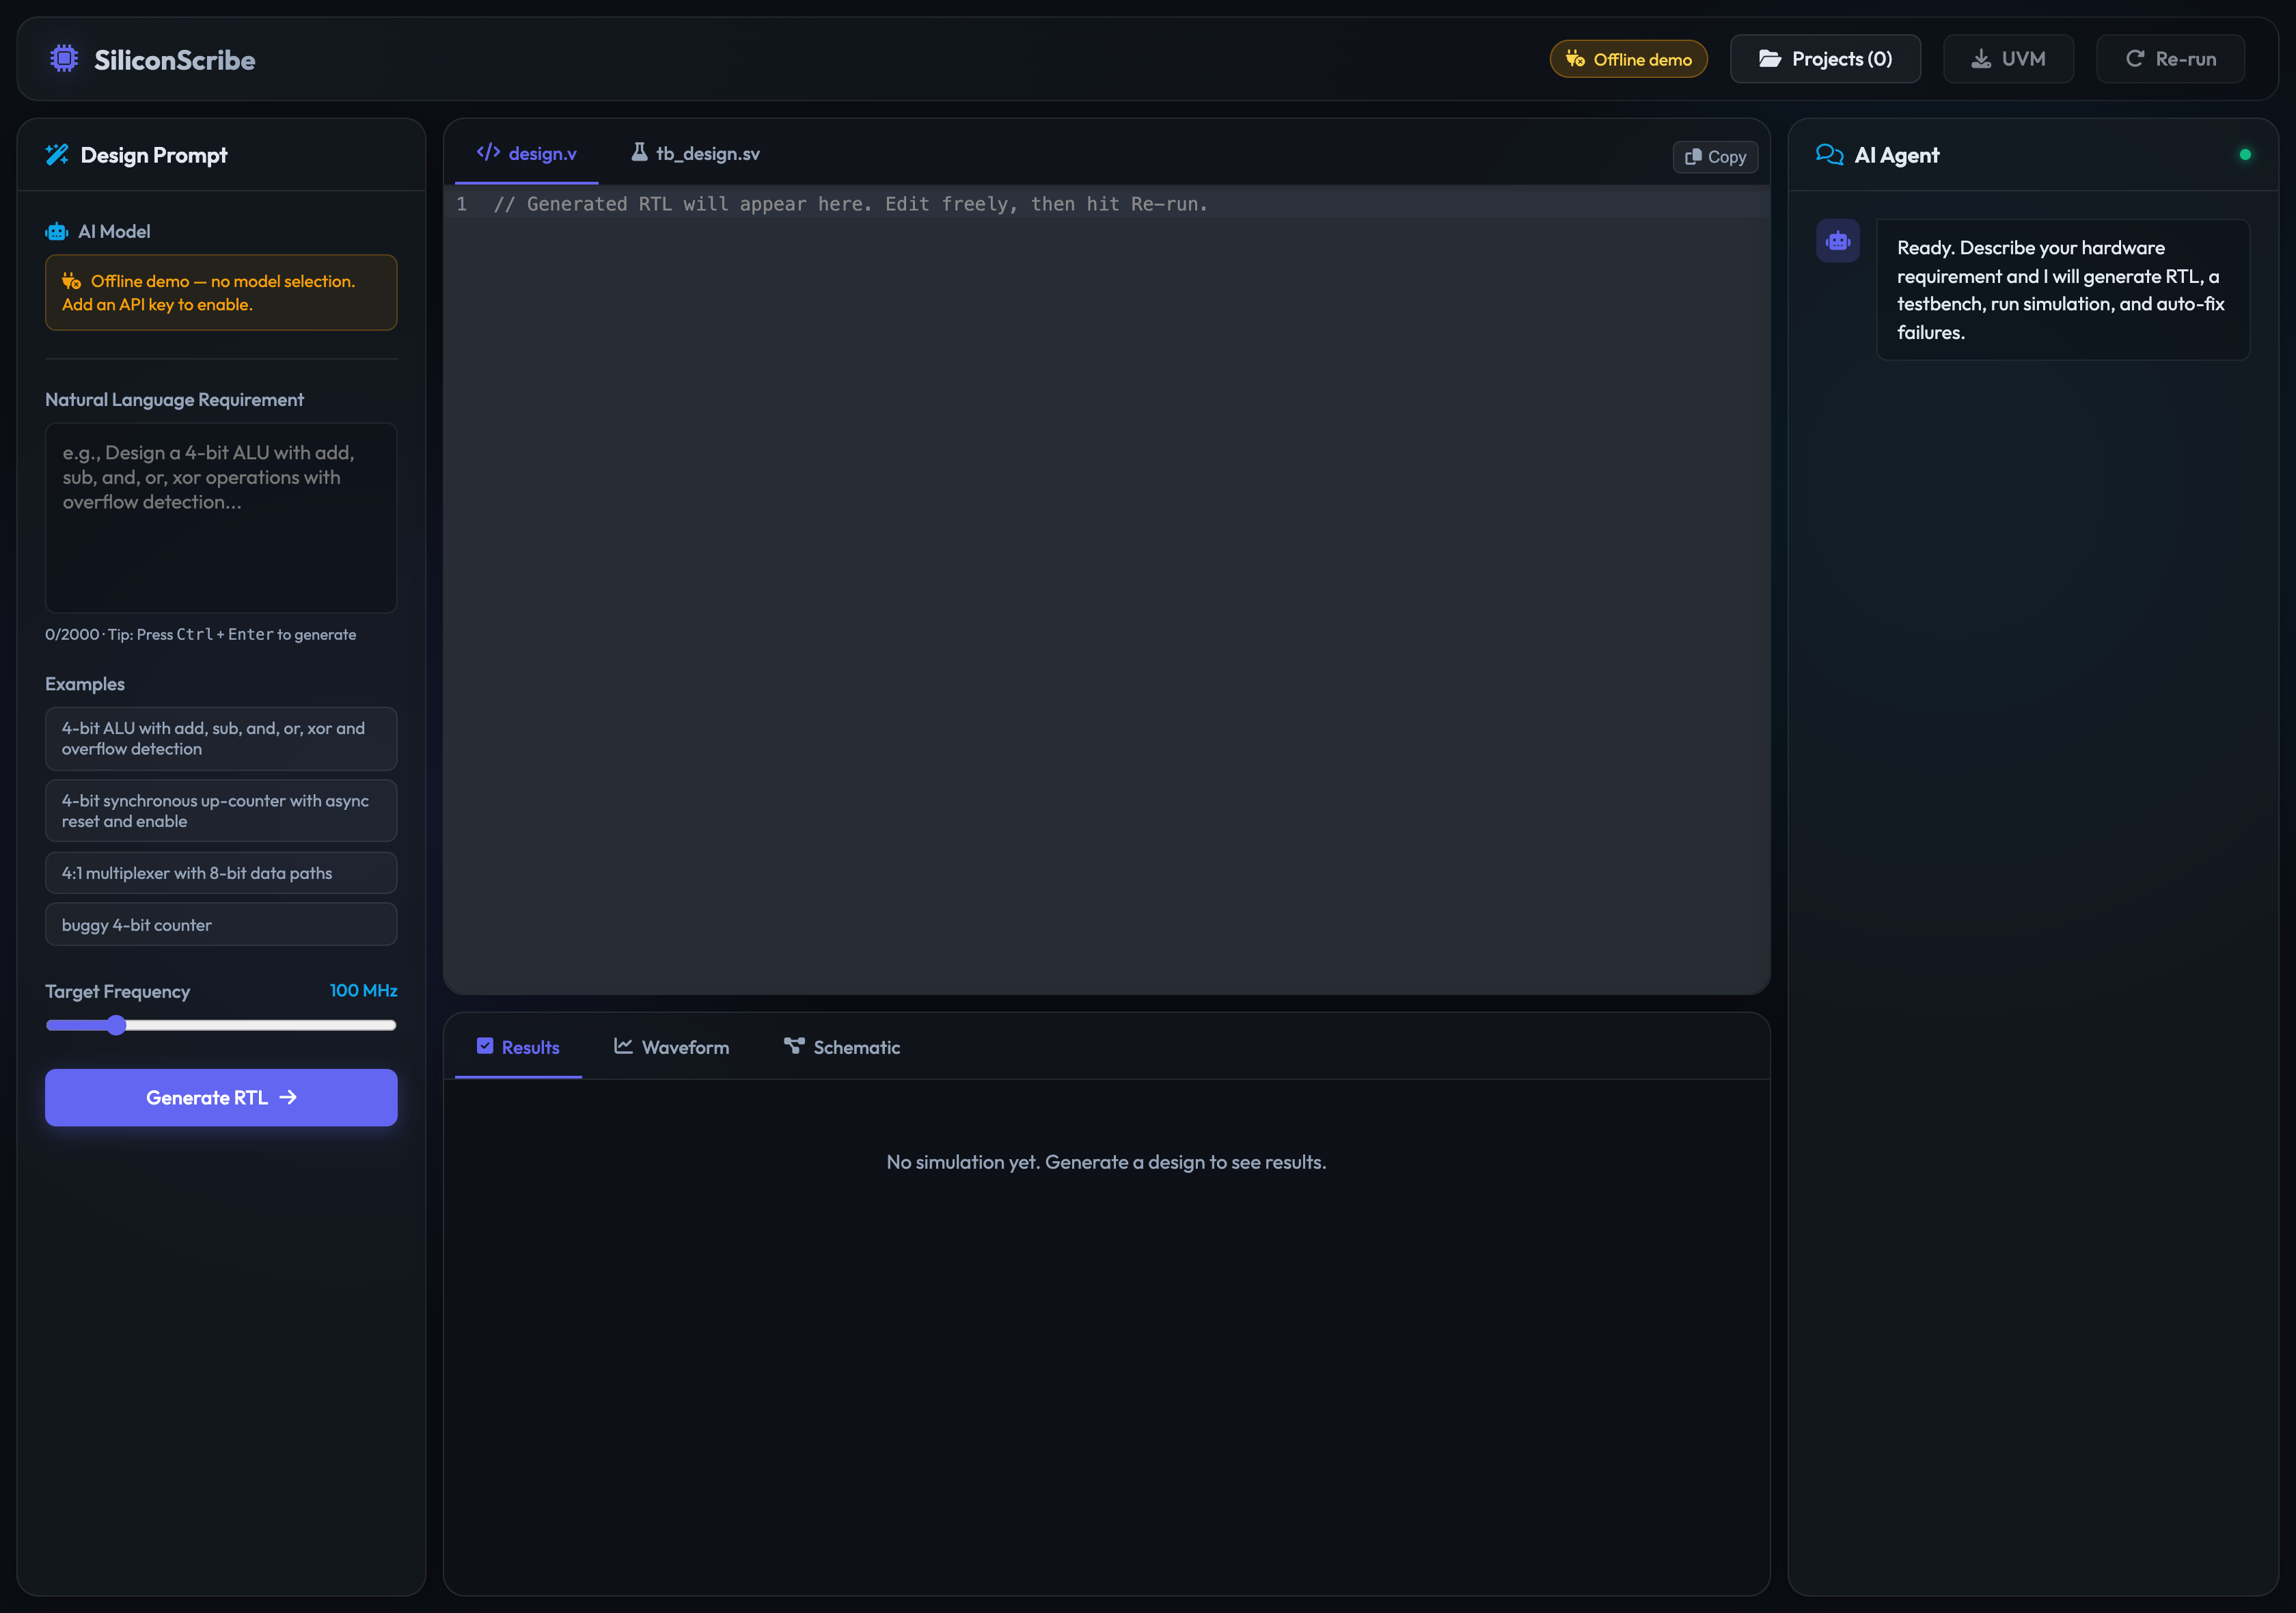
\includegraphics[width=0.60\textwidth]{15_home_screen.png}
\caption{Application home screen: design prompt with example chips, model selector and frequency hint (left), RTL and testbench editors with Results / Waveform / Schematic tabs (centre), and the live agent timeline (right). The amber badge shows the provider state; this capture is the offline demonstration mode.}
\label{fig:home}
\end{figure}

\subsection{Backend}
The FastAPI service exposes \code{/api/design/stream} (SSE),
\code{/api/design/run} (blocking JSON), \code{/api/simulation/run},
\code{/api/synthesis/run}, \code{/api/models}, \code{/api/projects},
\code{/api/uvm/export}, and health/status endpoints. Each
design runs in an isolated workspace directory named by a 32-character design ID;
paths are validated against a strict regular expression before any file operation. Generated Verilog is additionally screened by a sandbox policy (Section~\ref{sec:sandbox}) before it is compiled.
Rate limiting is per client IP. SQLite stores project metadata and the latest
result so the history drawer can reload a design.

\subsection{Provider Isolation}
The provider is selected from environment variables: \code{OFFLINE_MODE} forces the
curated provider; otherwise \code{OPENCODE_API_KEY}/\code{ZEN_API_KEY} selects
OpenCode Zen, \code{NVIDIA_API_KEY} selects NVIDIA NIM, and
\code{OPENAI_API_KEY}+\code{OPENAI_BASE_URL} selects any OpenAI-compatible
endpoint. The configured model is authoritative: if it is not in the curated
catalog, \code{/api/models} exposes \emph{only} that model. This prevents the UI
from selecting a model name the active gateway cannot serve --- a real defect found
during screenshot validation (Section~\ref{sec:discussion}).

\begin{figure}[t]
\centering
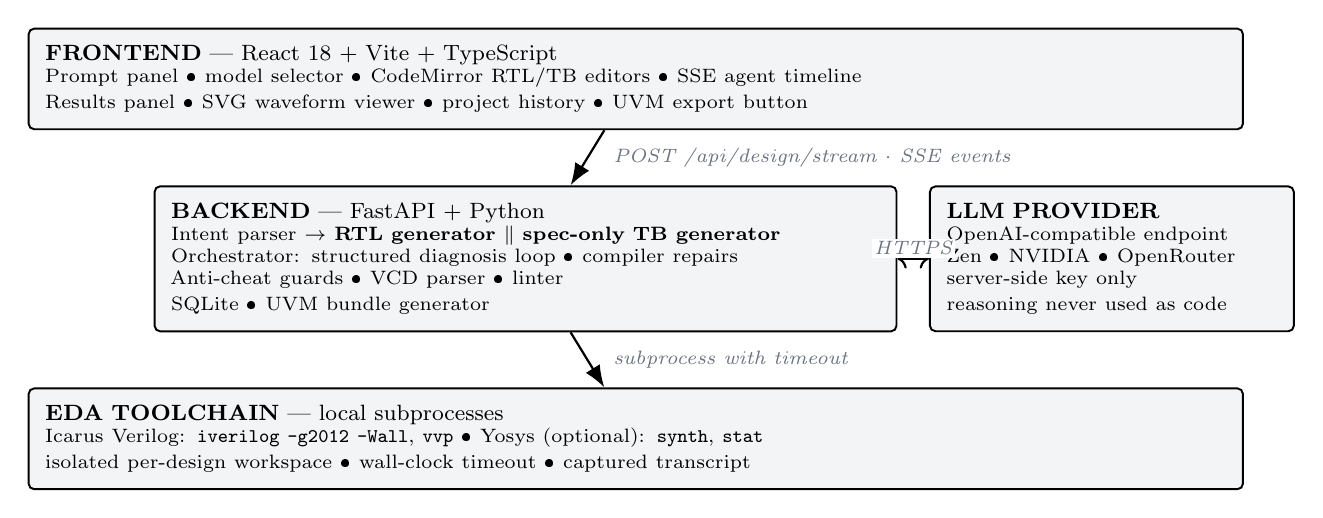
\begin{tikzpicture}[
    font=\footnotesize,
    tier/.style={draw=ink,line width=0.7pt,rounded corners=2pt,
                 fill=softgrey,align=left,
                 inner sep=6pt,minimum height=1.25cm},
    arr/.style={-{Latex[length=2.8mm]},line width=0.8pt,color=ink},
    lbl/.style={font=\scriptsize\itshape,color=rulegrey,align=center}
  ]
  \node[tier,text width=15.0cm] (fe) {\textbf{FRONTEND} --- React 18 + Vite + TypeScript\\
    \scriptsize Prompt panel \textbullet\ model selector \textbullet\ CodeMirror RTL/TB
    editors \textbullet\ SSE agent timeline\\
    \scriptsize Results panel \textbullet\ SVG waveform viewer \textbullet\ project
    history \textbullet\ UVM export button};
  \node[tier,text width=9.0cm,below=7mm of fe,xshift=-1.4cm] (be) {\textbf{BACKEND} --- FastAPI + Python\\
    \scriptsize Intent parser $\rightarrow$ \textbf{RTL generator} $\parallel$
    \textbf{spec-only TB generator}\\
    \scriptsize Orchestrator: structured diagnosis loop \textbullet\ compiler repairs\\
    \scriptsize Anti-cheat guards \textbullet\ VCD parser \textbullet\ linter\\
    \scriptsize SQLite \textbullet\ UVM bundle generator};
  \node[tier,text width=4.2cm,right=4mm of be] (llm) {\textbf{LLM PROVIDER}\\
    \scriptsize OpenAI-compatible endpoint\\
    \scriptsize Zen \textbullet\ NVIDIA \textbullet\ OpenRouter\\
    \scriptsize server-side key only\\
    \scriptsize reasoning never used as code};
  \node[tier,text width=15.0cm,below=7mm of be,xshift=1.4cm] (eda) {\textbf{EDA TOOLCHAIN} --- local
    subprocesses\\
    \scriptsize Icarus Verilog: \code{iverilog -g2012 -Wall}, \code{vvp}
    \textbullet\ Yosys (optional): \code{synth}, \code{stat}\\
    \scriptsize isolated per-design workspace \textbullet\ wall-clock timeout
    \textbullet\ captured transcript};
  \draw[arr] (fe) -- node[lbl,right=2mm]{POST /api/design/stream $\cdot$ SSE events} (be);
  \draw[arr] (be) -- node[lbl,right=2mm]{subprocess with timeout} (eda);
  \draw[arr,<->] (be.east) -- node[lbl,above,fill=white,inner sep=1pt]{HTTPS} (llm.west);
\end{tikzpicture}
\caption{Three-tier architecture. RTL and testbench generation are independent
branches of the same specification; only the simulator decides PASS/FAIL.}
\label{fig:arch}
\end{figure}

\subsection{Data Model}
All interfaces are typed with Pydantic (Table~\ref{tab:datamodel}); invalid requests are rejected with HTTP 422 before any work starts.

\begin{table}[H]
\centering
\caption{Core data structures (\texttt{backend/models.py}).}
\label{tab:datamodel}
\footnotesize
\begin{tabularx}{\textwidth}{@{}p{3.1cm}X@{}}
\toprule
\textbf{Model} & \textbf{Key fields} \\
\midrule
\code{RTLDesignSpec} & module name, parameters, ports, behaviour, constraints \\
\code{PortSpec} & name, direction (input/output/inout), width 1--1024, description \\
\code{RunRequest} & prompt ($\le$2000 chars), frequency hint, self-correct flag, max iterations 0--10, timeout 1--120\,s, model, reasoning effort \\
\code{SimulationResult} & status, test/pass/fail counts, coverage, structured errors, waveform and transcript paths, log excerpt \\
\code{IterationRecord} & iteration, status, fix summary, fix type, structured diagnosis, counts, log excerpt \\
\code{RunResponse} & spec, RTL, testbench, explanation, final result, iteration history, waveform, schematic, synthesis, fallback notice \\
\bottomrule
\end{tabularx}
\end{table}

\subsection{API Surface}
\begin{table}[H]
\centering
\caption{HTTP endpoints. All mutating and project routes are rate-limited to 20 requests per minute per client.}
\label{tab:api}
\footnotesize
\begin{tabularx}{\textwidth}{@{}l p{4.2cm} X@{}}
\toprule
\textbf{Method} & \textbf{Path} & \textbf{Purpose} \\
\midrule
POST & \code{/api/design/stream} & Full pipeline streamed as Server-Sent Events (used by the browser); persists the finished run \\
POST & \code{/api/design/run} & Same pipeline, single JSON response; persists the run \\
POST & \code{/api/simulation/run} & Simulate a hand-edited RTL/testbench pair once \\
POST & \code{/api/synthesis/run} & Yosys synthesis if installed, otherwise an explicit unavailable result \\
POST & \code{/api/uvm/export} & 16-file UVM bundle as a file map and zip \\
GET/DELETE & \code{/api/projects[/\{id\}]} & List, load or delete saved projects \\
GET & \code{/api/models} & Provider state and selectable models \\
POST & \code{/api/admin/cleanup} & Workspace garbage collection; disabled unless an admin token is configured \\
GET & \code{/}, \code{/health} & Status and simulator availability \\
\bottomrule
\end{tabularx}
\end{table}

\subsection{Event Protocol and Run Sequence}
The streaming route emits one JSON event per stage: \code{start}, \code{intent}, \code{rtl}, \code{lint}, \code{testbench}, \code{explanation}, \code{simulate}, \code{fixing}, \code{fix}, \code{synthesis}, and finally \code{done} with the complete \code{RunResponse}, or \code{error}. Figure~\ref{fig:seq} shows the interaction for one run.

\begin{figure}[H]
\centering
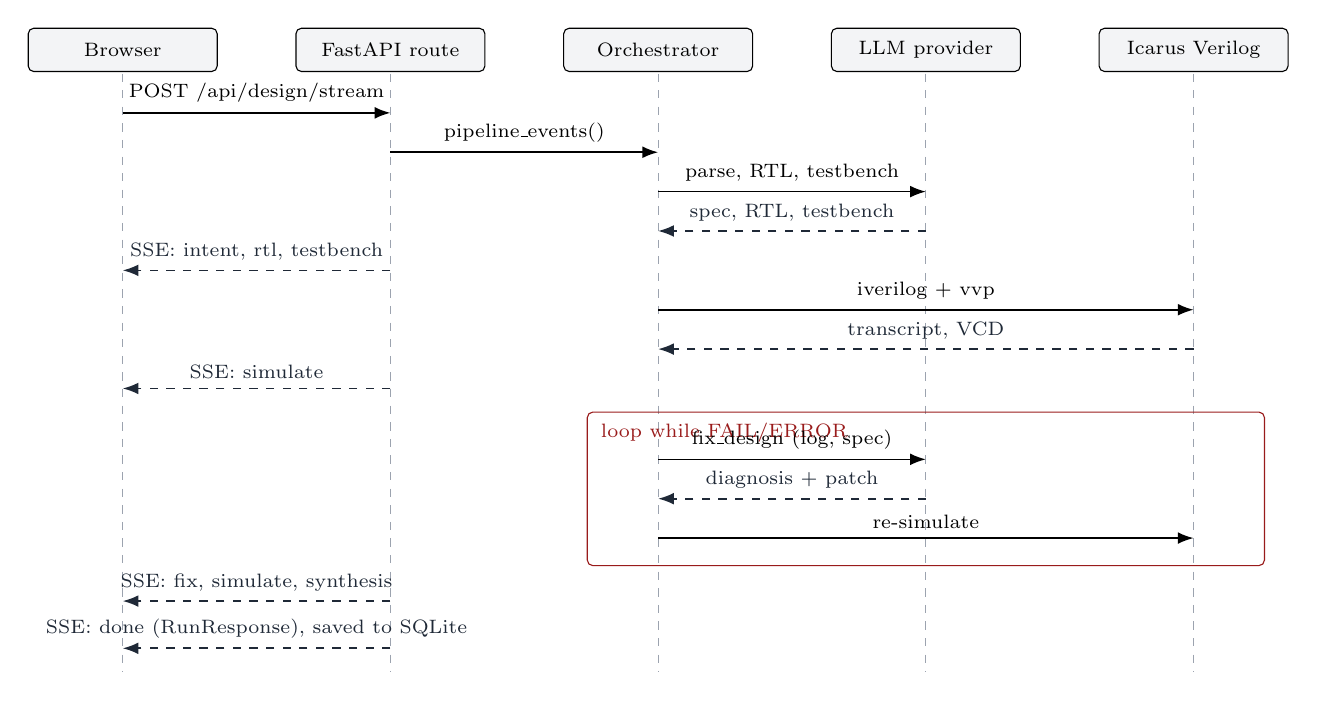
\begin{tikzpicture}[font=\scriptsize,
  actor/.style={draw=ink,fill=softgrey,rounded corners=2pt,minimum width=2.4cm,minimum height=0.55cm,align=center},
  msg/.style={-{Latex[length=2mm]},line width=0.6pt},
  ret/.style={-{Latex[length=2mm]},line width=0.6pt,dashed,color=inkdark}]
\foreach \x/\n in {0/Browser,3.4/FastAPI route,6.8/Orchestrator,10.2/LLM provider,13.6/Icarus Verilog}{
  \node[actor] at (\x,0) {\n};
  \draw[dashed,color=midgrey] (\x,-0.3) -- (\x,-7.9);}
\draw[msg] (0,-0.8) -- node[above]{POST /api/design/stream} (3.4,-0.8);
\draw[msg] (3.4,-1.3) -- node[above]{pipeline\_events()} (6.8,-1.3);
\draw[msg] (6.8,-1.8) -- node[above]{parse, RTL, testbench} (10.2,-1.8);
\draw[ret] (10.2,-2.3) -- node[above]{spec, RTL, testbench} (6.8,-2.3);
\draw[ret] (3.4,-2.8) -- node[above]{SSE: intent, rtl, testbench} (0,-2.8);
\draw[msg] (6.8,-3.3) -- node[above]{iverilog + vvp} (13.6,-3.3);
\draw[ret] (13.6,-3.8) -- node[above]{transcript, VCD} (6.8,-3.8);
\draw[ret] (3.4,-4.3) -- node[above]{SSE: simulate} (0,-4.3);
\draw[draw=failred,rounded corners=2pt] (5.9,-4.6) rectangle (14.5,-6.55);
\node[anchor=north west,color=failred] at (5.95,-4.62) {loop while FAIL/ERROR};
\draw[msg] (6.8,-5.2) -- node[above]{fix\_design (log, spec)} (10.2,-5.2);
\draw[ret] (10.2,-5.7) -- node[above]{diagnosis + patch} (6.8,-5.7);
\draw[msg] (6.8,-6.2) -- node[above]{re-simulate} (13.6,-6.2);
\draw[ret] (3.4,-7.0) -- node[above]{SSE: fix, simulate, synthesis} (0,-7.0);
\draw[ret] (3.4,-7.6) -- node[above]{SSE: done (RunResponse), saved to SQLite} (0,-7.6);
\end{tikzpicture}
\caption{Sequence of one streamed run. Guards inside the loop can stop it early (Figure~\ref{fig:loop}).}
\label{fig:seq}
\end{figure}

\subsection{Persistence Schema}
Projects are stored in one SQLite table with columns \code{id}, \code{prompt}, \code{module_name}, \code{rtl_spec}, \code{rtl_code}, \code{testbench_code}, \code{explanation}, \code{status}, \code{pass_count}, \code{fail_count}, \code{iterations}, \code{created_at}, \code{waveform_truncated} and a JSON \code{data} column holding the full response. Every call opens its own connection, so the thread-pooled routes do not share connection state.

\subsection{Security Design}
\label{sec:security}
\begin{itemize}
\item \textbf{Input limits:} prompt 2000 characters, RTL/testbench 50\,000 characters, 200\,KB per written file, timeouts 1--120\,s, iterations 0--10, identifiers validated by regular expression.
\item \textbf{Path safety:} design IDs match \code{^[a-zA-Z0-9_-]\{1,32\}$}; every path is resolved and checked to stay inside the workspace, including through symbolic links.
\item \textbf{Execution:} compile timeout 30\,s, simulation timeout, sandbox policy, scrubbed environment and output-size cap (Section~\ref{sec:sandbox}).
\item \textbf{Abuse control:} per-IP sliding-window rate limit; admin cleanup requires a token compared in constant time.
\item \textbf{Information hygiene:} internal errors return a generic message; API keys stay server-side and are never logged; CORS is restricted to known origins plus Vercel preview deployments.
\end{itemize}

% ========================================================== 3. METHOD ======
\section{Methodology}
\label{sec:method}

\subsection{Specification Parsing}
The first live call converts the prompt into an \code{RTLDesignSpec}: module name,
parameters, ports (name, direction, width, description), behavioural rules, and
constraints. The parser prompt requires the specification to pin down every
observable behaviour, including reset polarity, opcode tables, priority order, and
the value of all outputs for all input combinations. This is essential because the
RTL and testbench generators never see each other's output.

\subsection{Independent, Specification-Derived Testbenches}
\label{sec:tb}
The testbench generator receives only the parsed specification --- the RTL body is
withheld. This breaks the circular verification of the earlier progress report, in
which the same model could write a DUT and a testbench that were consistently wrong
together. The prompt requires:

\begin{itemize}
\item a top module named \code{testbench}, with explicit named port connections;
\item clock/reset generation for sequential DUTs;
\item directed corner cases \emph{and} at least 100 randomized vectors;
\item expected values computed from the specification, compared with \code{===};
\item integer \code{pass_count}/\code{fail_count} and exact summary lines;
\item \code{\$dumpfile}/\code{\$dumpvars} for the waveform;
\item Verilog-2001/Icarus compatibility: module-scope declarations only, no
\code{break}, \code{continue}, \code{return}, or \code{disable}; a first-match
\code{if/else-if} chain or a \code{found} flag for priority logic; width-correct
comparisons.
\end{itemize}

These rules were not written speculatively. Each one corresponds to a real failure
observed in a live run (Section~\ref{sec:discussion}).

\subsection{Execution}
The orchestrator writes \code{design.sv} and \code{testbench.sv} into the workspace,
compiles with \code{iverilog -g2012 -Wall -o testbench.vvp}, and runs
\code{vvp} under a configurable wall-clock timeout. The simulator output is parsed
for the exact \code{Passed:}/\code{Failed:} lines and the \code{ALL TESTS PASSED}
marker. Compilation diagnostics are parsed into structured errors. PASS/FAIL is
decided by this execution, never by model text.

\subsection{Execution Sandbox Policy}
\label{sec:sandbox}
Generated or user-edited Verilog is executed by \code{vvp} with the server's privileges, so it is untrusted input. The final-review probe (Section~\ref{sec:review}) showed that Verilog file-I/O system tasks (\code{$fopen}, \code{$fgets}, \code{$fwrite}, \code{$readmemh} and related tasks) could read or write any path the process could reach, and that the contents came back in the API response. Three independent controls now apply to every simulation:

\begin{enumerate}[label=\textbf{\arabic*.}]
\item \textbf{Static policy.} Before anything is compiled, the RTL and testbench are scanned and rejected if they use file or process system tasks, the include directive, macro token pasting, or a \code{$dumpfile} argument that is not a plain file name. The scan deliberately does not strip comments: a naive comment stripper can be fooled by a double slash inside a string literal into hiding a forbidden call.
\item \textbf{Scrubbed environment.} The compiler and simulator run with a minimal environment (path, locale and temporary directory only), so API keys held by the server never reach them.
\item \textbf{Output cap.} The simulator runs under a file-size limit, so a runaway \code{$display} loop cannot fill the disk before the wall-clock timeout.
\end{enumerate}

This is defence in depth, not a security boundary: a static scan of a language as flexible as Verilog can never be airtight. For multi-user deployment the simulator must run inside a container or jail (Section~\ref{sec:scale}).

\subsection{Structured Diagnosis and Repair}
\label{sec:loop}
When the result is FAIL or ERROR, the fixer receives the RTL, the testbench, the
specification, and the simulator log. It must answer in explicit sections:

\begin{lstlisting}[language=,basicstyle=\ttfamily\scriptsize]
<diagnosis>
symptom: <what the log shows, with the first failing vector>
root_cause: <the hardware reason, not a restatement of the symptom>
fix_location: <file / module / line / signal>
confidence: high|medium|low
</diagnosis>
<rtl> ... complete corrected RTL ... </rtl>
<testbench> ... complete testbench ... </testbench>
<summary> ... one sentence ... </summary>
\end{lstlisting}

The section format replaced a fragile JSON response after a live run produced
malformed JSON with unescaped Verilog newlines and quotes. A tolerant JSON path and
a field-salvage path remain for older models, but compliant models use the section
format.

The fixer is explicitly instructed to check the \emph{testbench oracle} against the
specification: if the RTL matches the spec but the expected-value logic does not,
the bug is in the testbench. This is a real failure mode: one generated testbench
concatenated a 32-bit integer with a 3-bit code, making a 35-bit comparison that
could never equal the 4-bit DUT output.

Figure~\ref{fig:loop} shows the control flow. A patch is rejected if it removes
self-checks from a testbench that already compiled and ran. The loop also tracks a
comment/whitespace-normalised hash of \emph{both} RTL and testbench; an unchanged
state is a no-op, and a repeated state is oscillation. Both terminate the loop
instead of burning tokens.


\subsection{Deterministic Compiler Repairs}
Some failures are not design decisions and should not be delegated to a model:

\begin{itemize}
\item \textbf{wire$\rightarrow$reg.} Icarus reports
\code{X is not a valid l-value} when a net is assigned from a procedural block. The
repair is scoped to the file named in the diagnostic, changes only that declaration,
and is recorded as \code{fix_type="compiler_repair"} with a real diagnosis.
\item \textbf{disable$\rightarrow$return.} Icarus rejects \code{disable <function>}
inside a function but accepts \code{return <function>}. The repair preserves the
first-match semantics of the oracle.
\end{itemize}

Neither repair touches the testbench's checks; both are labelled as compiler
repairs in the UI and in \code{iteration_history}.

\subsection{Honest Degraded Mode}
\label{sec:fallback}
The offline curated designs remain available for demonstrations and for the
automated suite, but the policy is explicit:

\begin{itemize}
\item If the provider is unreachable \emph{before any live artifact exists}, the
pipeline may fall back to a curated design and attaches a visible
\code{fallback_notice}. The UI shows a degraded-mode banner.
\item Once a live call has succeeded, a later outage raises an error. The run does
not silently swap the user's design mid-flight.
\item Scripted offline fixes return \code{diagnosis=None} and
\code{fix_type="offline_scripted"}. They never fabricate a root cause.
\end{itemize}

This policy was added after an early live run silently switched to a curated design
when the provider failed, producing a PASS that did not correspond to the prompt.

\begin{figure}[H]
\centering
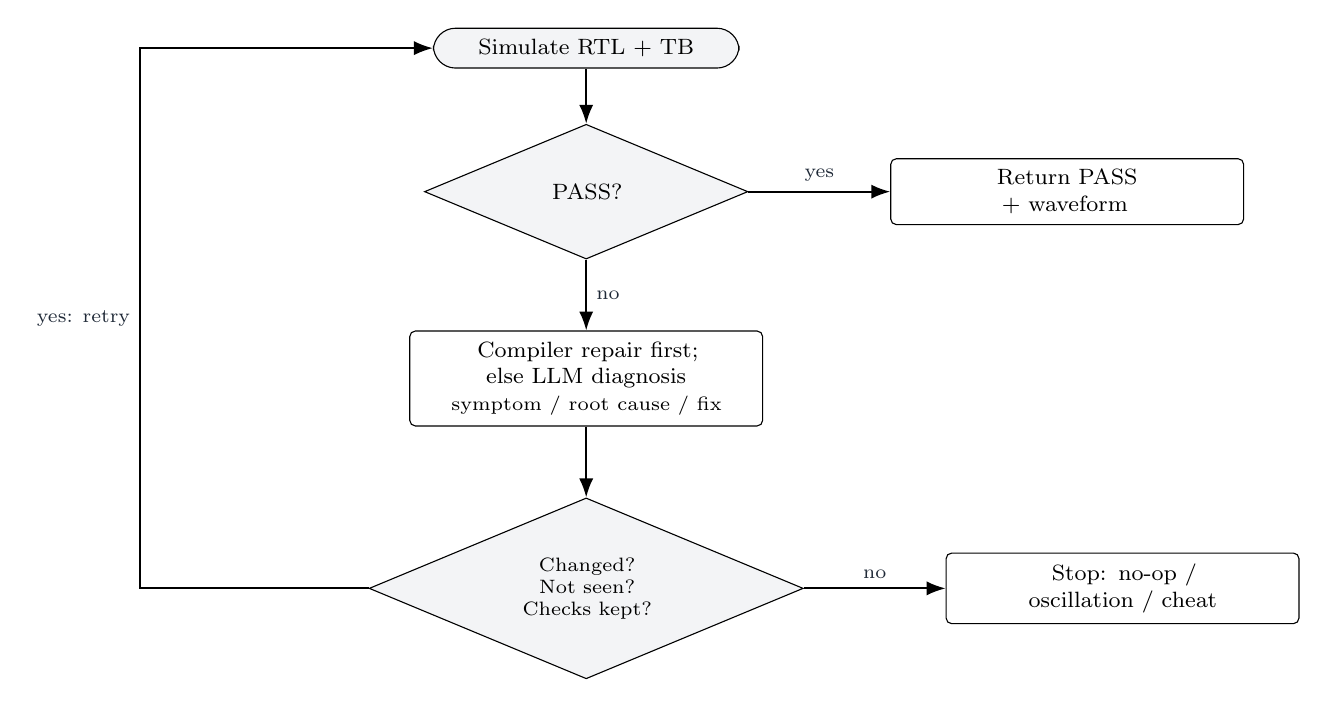
\begin{tikzpicture}[
    font=\footnotesize,
    start/.style={draw=ink,rounded corners=8pt,fill=softgrey,text width=3.6cm,align=center,inner sep=4pt},
    proc/.style={draw=ink,rounded corners=2pt,fill=white,text width=4.2cm,align=center,inner sep=4pt},
    dec/.style={draw=ink,diamond,aspect=2.4,fill=softgrey,text width=3.4cm,align=center,inner sep=1pt},
    arr/.style={-{Latex[length=2.4mm]},line width=0.7pt},
    lbl/.style={font=\scriptsize,color=inkdark}
  ]
  \node[start] (sim) {Simulate RTL + TB};
  \node[dec,below=7mm of sim] (ok) {PASS?};
  \node[proc,below=9mm of ok] (diag) {Compiler repair first;\\else LLM diagnosis\\
    \scriptsize symptom / root cause / fix};
  \node[dec,below=9mm of diag,font=\scriptsize] (guard) {Changed?\\Not seen?\\Checks kept?};
  \node[proc,right=18mm of ok] (done) {Return PASS\\+ waveform};
  \node[proc,right=18mm of guard] (stop) {Stop: no-op /\\oscillation / cheat};
  \draw[arr] (sim) -- (ok);
  \draw[arr] (ok) -- node[lbl,above]{yes} (done);
  \draw[arr] (ok) -- node[lbl,right]{no} (diag);
  \draw[arr] (diag) -- (guard);
  \draw[arr] (guard) -- node[lbl,above]{no} (stop);
  \draw[arr] (guard.west) -- ++(-2.9,0) |- node[lbl,left,pos=0.25]{yes: retry} (sim.west);
\end{tikzpicture}
\caption{Diagnosis and repair loop. Mechanical compiler repairs run before the LLM;
the simulator is the only oracle. A patch that removes testbench checks, changes
nothing, or repeats a previous state terminates the loop.}
\label{fig:loop}
\end{figure}


\subsection{Orchestration Algorithm}
\begin{lstlisting}[language=,basicstyle=\ttfamily\scriptsize,caption={Self-correction loop as implemented in orchestrator.py (simplified).},label={lst:algo}]
spec   = parse_intent(prompt)            # offline fallback only before any live call
rtl    = generate_rtl(spec)              # must contain a complete module; one retry
tb     = generate_testbench(spec)        # RTL withheld; must instantiate DUT and self-check
result = simulate(rtl, tb); seen = {hash(rtl, tb)}
for i in 1..max_iterations while result in {FAIL, ERROR}:
    if result == ERROR and compiler_repair applies:      # wire->reg, disable->return
        apply repair; result = simulate(rtl, tb); continue
    fix = fix_design(rtl, tb, log, spec)                  # diagnosis + full patched files
    if result != ERROR and checks(fix.tb) < checks(tb):   # anti-cheat
        fix.tb = tb
    h = hash(fix.rtl, fix.tb)                             # whitespace/comment-insensitive
    if h == hash(rtl, tb): stop("no-op")
    if h in seen:          stop("oscillation")
    seen.add(h); rtl, tb = fix.rtl, fix.tb; result = simulate(rtl, tb)
return result, history, waveform, schematic, synthesis
\end{lstlisting}

% ========================================================== 4. IMPL =======
\section{Implementation}
\label{sec:impl}

\begin{table}[H]
\centering
\caption{Principal implementation modules (all paths under \texttt{backend/} or
\texttt{frontend/src/}).}
\label{tab:modules}
\footnotesize
\begin{tabularx}{\textwidth}{@{}p{3.4cm}p{7.2cm}X@{}}
\toprule
\textbf{Module} & \textbf{Responsibility} & \textbf{Key idea} \\
\midrule
\code{main.py} & FastAPI routes, SSE streaming, rate limiting & one event stream per design \\
\code{orchestrator.py} & pipeline, repair loop, guards, fallback policy & simulator decides; anti-cheat \\
\code{llm_service.py} & provider config, prompts, fix parser, model listing, per-stage model routing & spec-only TB; section protocol \\
\code{simulator.py} & workspace, iverilog/vvp, log parsing, sandbox policy & isolated, timed, policy-screened execution \\
\code{vcd_parser.py} & VCD $\rightarrow$ JSON waveform & bounded size, hex buses \\
\code{linter.py} & Verilator $\rightarrow$ Icarus $\rightarrow$ regex & graceful degradation \\
\code{synthesis.py} & Yosys wrapper & optional; honest unavailable state \\
\code{db.py} & SQLite persistence, project retrieval & zero-dependency storage \\
\code{uvm_templates.py} & 16-file UVM 1.2 bundle & export-only, CI file-count check \\
\code{App.tsx} & SSE client, project state, export & live timeline, fallback banner \\
\code{ResultsPanel.tsx} & PASS/FAIL, metrics, diagnosis timeline & iteration history \\
\code{WaveformViewer.tsx} & SVG waveform & zoom, ruler, hex labels \\
\code{tools/mutation_sweep.py} & 14-mutant sweep over the curated designs & reproduces the kill rate \\
\bottomrule
\end{tabularx}
\end{table}

The backend is Python 3.14 with FastAPI, Pydantic, and the OpenAI Python client
pointed at an OpenAI-compatible base URL. The frontend is React 18, TypeScript,
Vite, and CodeMirror. Icarus Verilog 12.0 is the simulator. Yosys is optional; if
it is absent, the API returns \code{available:false} and the UI says so instead of
inventing cell counts.

\subsection{Test Strategy}
The backend suite has 100 tests: models and validation, linter behaviour, simulator
and VCD parsing, API edge cases, orchestrator repair/fallback/guard paths, LLM
response parsing (XML sections, malformed JSON salvage, literal newlines), and
verification-quality mutation tests (16 mutants), sandbox-policy tests, per-stage model-routing tests and a persistence test for the streaming route. The suite runs against a throw-away workspace and never touches the developer's database. The frontend suite has 38 vitest tests across
PromptPanel, ResultsPanel, and WaveformViewer. The mutation tests are the important
ones: they take a curated design, inject a semantic bug (wrong increment, missing
reset, wrong mux select, wrong ALU opcode), and assert that the independent
testbench reports FAIL. A testbench that cannot fail is not evidence.

\subsection{Technology Stack}
\begin{table}[H]
\centering
\caption{Technology stack on the validation machine (Apple M4, macOS).}
\label{tab:stack}
\footnotesize
\begin{tabularx}{\textwidth}{@{}p{2.4cm}X@{}}
\toprule
\textbf{Layer} & \textbf{Components} \\
\midrule
Backend & Python 3.14.2, FastAPI, Uvicorn, Pydantic 2, OpenAI Python client (pinned in \code{requirements.txt}; the machine ran FastAPI 0.141.1, Pydantic 2.13.5) \\
Frontend & React 18.3, TypeScript 5.7, Vite 6, CodeMirror 6, Vitest 4 with Testing Library and jsdom \\
EDA & Icarus Verilog 12.0; Yosys and Verilator optional (not installed on this machine) \\
Operations & Docker multi-stage image, Docker Compose, GitHub Actions CI, Vercel (frontend) and Render (backend) free tiers \\
\bottomrule
\end{tabularx}
\end{table}

% ========================================================== TESTING =======
\section{Testing and Quality Assurance}
\label{sec:testing}

\subsection{Strategy}
Testing works at six levels: unit tests of each module; integration tests of the pipeline with real Icarus runs; mutation tests that prove the testbenches can fail; security tests of the sandbox policy; live validation against a real model; and automated browser captures of the running interface. The backend suite runs against a throw-away workspace, so it never touches the developer's database.

\subsection{Test inventory}
\begin{table}[H]
\centering
\caption{Automated tests (100 backend, 38 frontend), all passing.}
\label{tab:tests}
\footnotesize
\begin{tabularx}{\textwidth}{@{}p{4.8cm}r X@{}}
\toprule
\textbf{File} & \textbf{Tests} & \textbf{Covers} \\
\midrule
\code{test_sandbox.py} & 18 & sandbox policy, end-to-end file-access block, environment scrub, output cap \\
\code{test_verification_quality.py} & 17 & 16 semantic mutants plus self-check detection \\
\code{test_orchestrator.py} & 15 & repair loop, compiler repairs, guards, fallback policy \\
\code{test_linter.py} & 11 & tool and heuristic lint paths \\
\code{test_llm_parsing.py} & 9 & section protocol, malformed JSON salvage, code extraction \\
\code{test_edge_cases.py} & 6 & limits, timeouts, malformed inputs \\
\code{test_vcd_parser.py} & 6 & VCD parsing, truncation, x/z handling \\
\code{test_api.py} & 5 & routes, streaming, rate limit \\
\code{test_model_routing.py} & 5 & per-stage model routing and precedence \\
\code{test_simulator.py} & 5 & compile, run, verdict parsing \\
\code{test_models.py} & 2 & data-model validation \\
\code{test_stream_persistence.py} & 1 & streamed run saved and listed \\
\midrule
Frontend (Vitest) & 38 & ResultsPanel (18), WaveformViewer (11), PromptPanel (9) \\
\bottomrule
\end{tabularx}
\end{table}

\subsection{Verdict rules under test}
The simulator verdict is deterministic: any \code{Failed: N} with $N>0$ gives FAIL; a runtime error without the pass marker gives ERROR; \code{ALL TESTS PASSED} or a positive pass count gives PASS; a missing summary gives ERROR so the loop can react; and a run exceeding its timeout gives TIMEOUT. Compile failures are parsed into file/line errors and returned as ERROR.

\subsection{Continuous integration}
Every push runs three jobs: the backend job installs Icarus and Yosys, runs Ruff lint, the test suite, a UVM bundle check and an end-to-end smoke run; the frontend job type-checks, runs Vitest and builds; and a Docker job builds the image.

\subsection{Pipeline performance}
\label{sec:perf}
Table~\ref{tab:perf} gives medians measured on the validation machine (Apple M4) in offline mode, so they exclude model latency. Live runs add the provider's response time for each of the four or five model calls, which dominates end-to-end time.

\begin{table}[H]
\centering
\caption{Measured local performance (median; 7 runs for simulation, 5 for the pipeline).}
\label{tab:perf}
\small
\begin{tabular}{@{}l r l r@{}}
\toprule
\textbf{Design} & \textbf{Checks} & \textbf{Operation} & \textbf{Median} \\
\midrule
full adder & 8 & compile + simulate & 22 ms \\
4:1 mux & 100 & compile + simulate & 22 ms \\
counter & 27 & compile + simulate & 25 ms \\
4-bit / 8-bit ALU & 200 & compile + simulate & 22 / 21 ms \\
counter, ALU, mux & -- & full offline pipeline & 45 ms \\
buggy counter & 27 & pipeline with one repair & 75 ms \\
\bottomrule
\end{tabular}
\end{table}

% ========================================================== 5. RESULTS ====
\section{Results}
\label{sec:results}

\subsection{Verification Matrix}
\begin{table}[H]
\centering
\caption{Final verification status on the development machine (macOS, 6 Nov 2026).}
\label{tab:verify}
\small
\begin{tabular}{@{}l l r l@{}}
\toprule
\textbf{Check} & \textbf{Command} & \textbf{Result} & \textbf{Status} \\
\midrule
Backend suite & \code{pytest tests/ -q} & 100 passed & \textcolor{passgreen}{\textbf{PASS}} \\
Frontend unit tests & \code{npx vitest run} & 38 passed & \textcolor{passgreen}{\textbf{PASS}} \\
TypeScript & \code{npx tsc -b} & 0 errors & \textcolor{passgreen}{\textbf{PASS}} \\
Production build & \code{npm run build} & 58 modules, 590 kB & \textcolor{passgreen}{\textbf{PASS}} \\
Icarus Verilog & \code{iverilog -V} & version 12.0 & available \\
Yosys & \code{yosys -V} & not installed & graceful unavailable \\
\bottomrule
\end{tabular}
\end{table}

The backend suite runs with Icarus on \code{PATH}; no simulator tests are skipped.
The tests that exercise the repair loop use real \code{iverilog}/\code{vvp}
execution in temporary workspaces.

\subsection{Live End-to-End Run: Arbitrary Priority-Encoder Prompt}
The following prompt was submitted to the running browser application and to a
headless harness using the same pipeline:

\begin{quote}
\itshape ``Design an 8-to-3 priority encoder with an active-high valid output. Input
in[7:0]; outputs code[2:0] and valid. The highest set bit wins: bit 7 $\rightarrow$
code 7, bit 6 $\rightarrow$ code 6, \ldots, bit 0 $\rightarrow$ code 0. When in is
zero, code=0 and valid=0. Purely combinational.''
\end{quote}

Live provider: OpenRouter, model \code{nvidia/nemotron-3-ultra-550b-a55b:free},
timeout 180~s, reasoning disabled. The UI run produced \textbf{105/105 checks,
0 failed, 100\% pass rate, PASS, 0 repair iterations}, with no degraded-mode
banner (Figure~\ref{fig:pass}). A second headless run of the same prompt produced
\textbf{116/116 checks} (the generated random loop bound differs slightly between
runs), also PASS on the first attempt. The model generated a \code{casez} priority
chain; the independent testbench combined directed corner cases with randomized
vectors (16 directed cases and 100 random vectors in the archived testbench). The exact RTL is shown in Listing~\ref{lst:rtl}.

\begin{lstlisting}[caption={RTL generated live for the priority encoder (excerpt).},
                   label={lst:rtl}]
module priority_encoder_8to3 (
    input  wire [7:0] in,
    output reg  [2:0] code,
    output reg        valid
);
    always @(*) begin
        code = 3'd0; valid = 1'b0;
        casez (in)
            8'b1???????: begin code = 3'd7; valid = 1'b1; end
            8'b01??????: begin code = 3'd6; valid = 1'b1; end
            8'b001?????: begin code = 3'd5; valid = 1'b1; end
            8'b0001????: begin code = 3'd4; valid = 1'b1; end
            8'b00001???: begin code = 3'd3; valid = 1'b1; end
            8'b000001??: begin code = 3'd2; valid = 1'b1; end
            8'b0000001?: begin code = 3'd1; valid = 1'b1; end
            8'b00000001: begin code = 3'd0; valid = 1'b1; end
            default:     begin code = 3'd0; valid = 1'b0; end
        endcase
    end
endmodule
\end{lstlisting}

\begin{figure}[H]
\centering
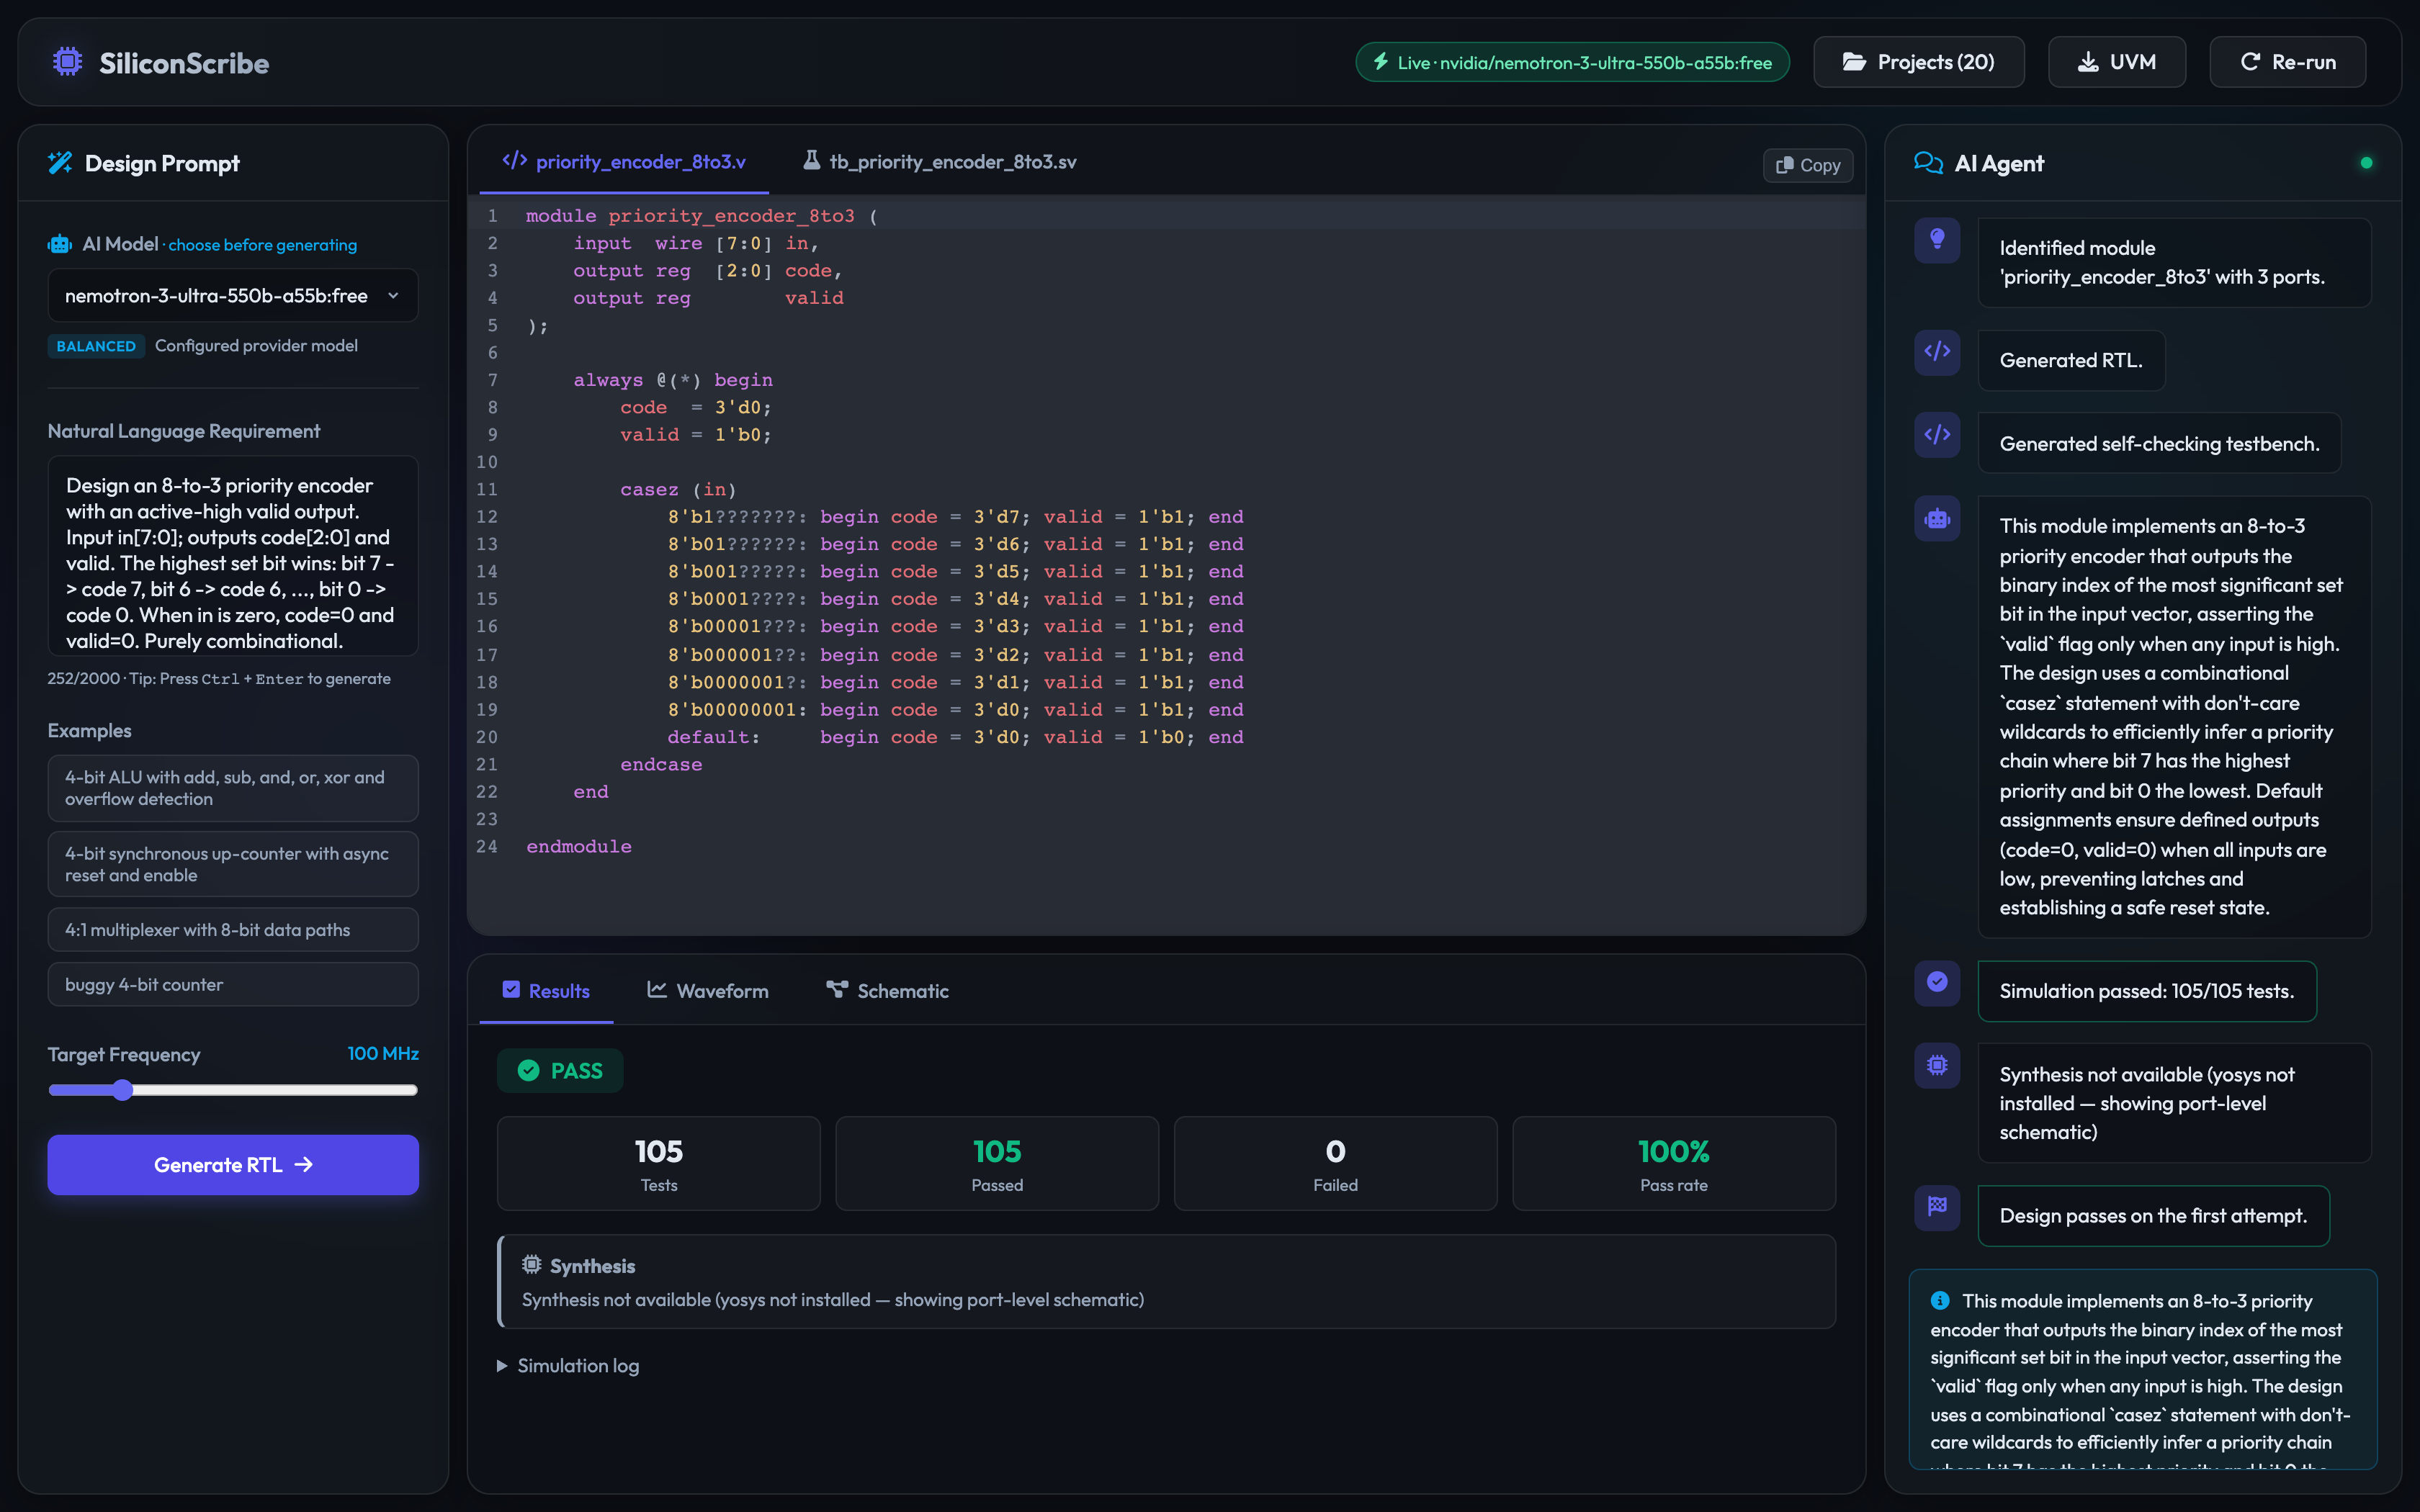
\includegraphics[width=0.78\textwidth]{03_live_pass_results.png}
\caption{Live browser run: arbitrary priority-encoder prompt, PASS, 105/105 checks,
100\% pass rate, no degraded-mode banner. The configured model is shown in the
prompt panel.}
\label{fig:pass}
\end{figure}

\begin{figure}[H]
\centering
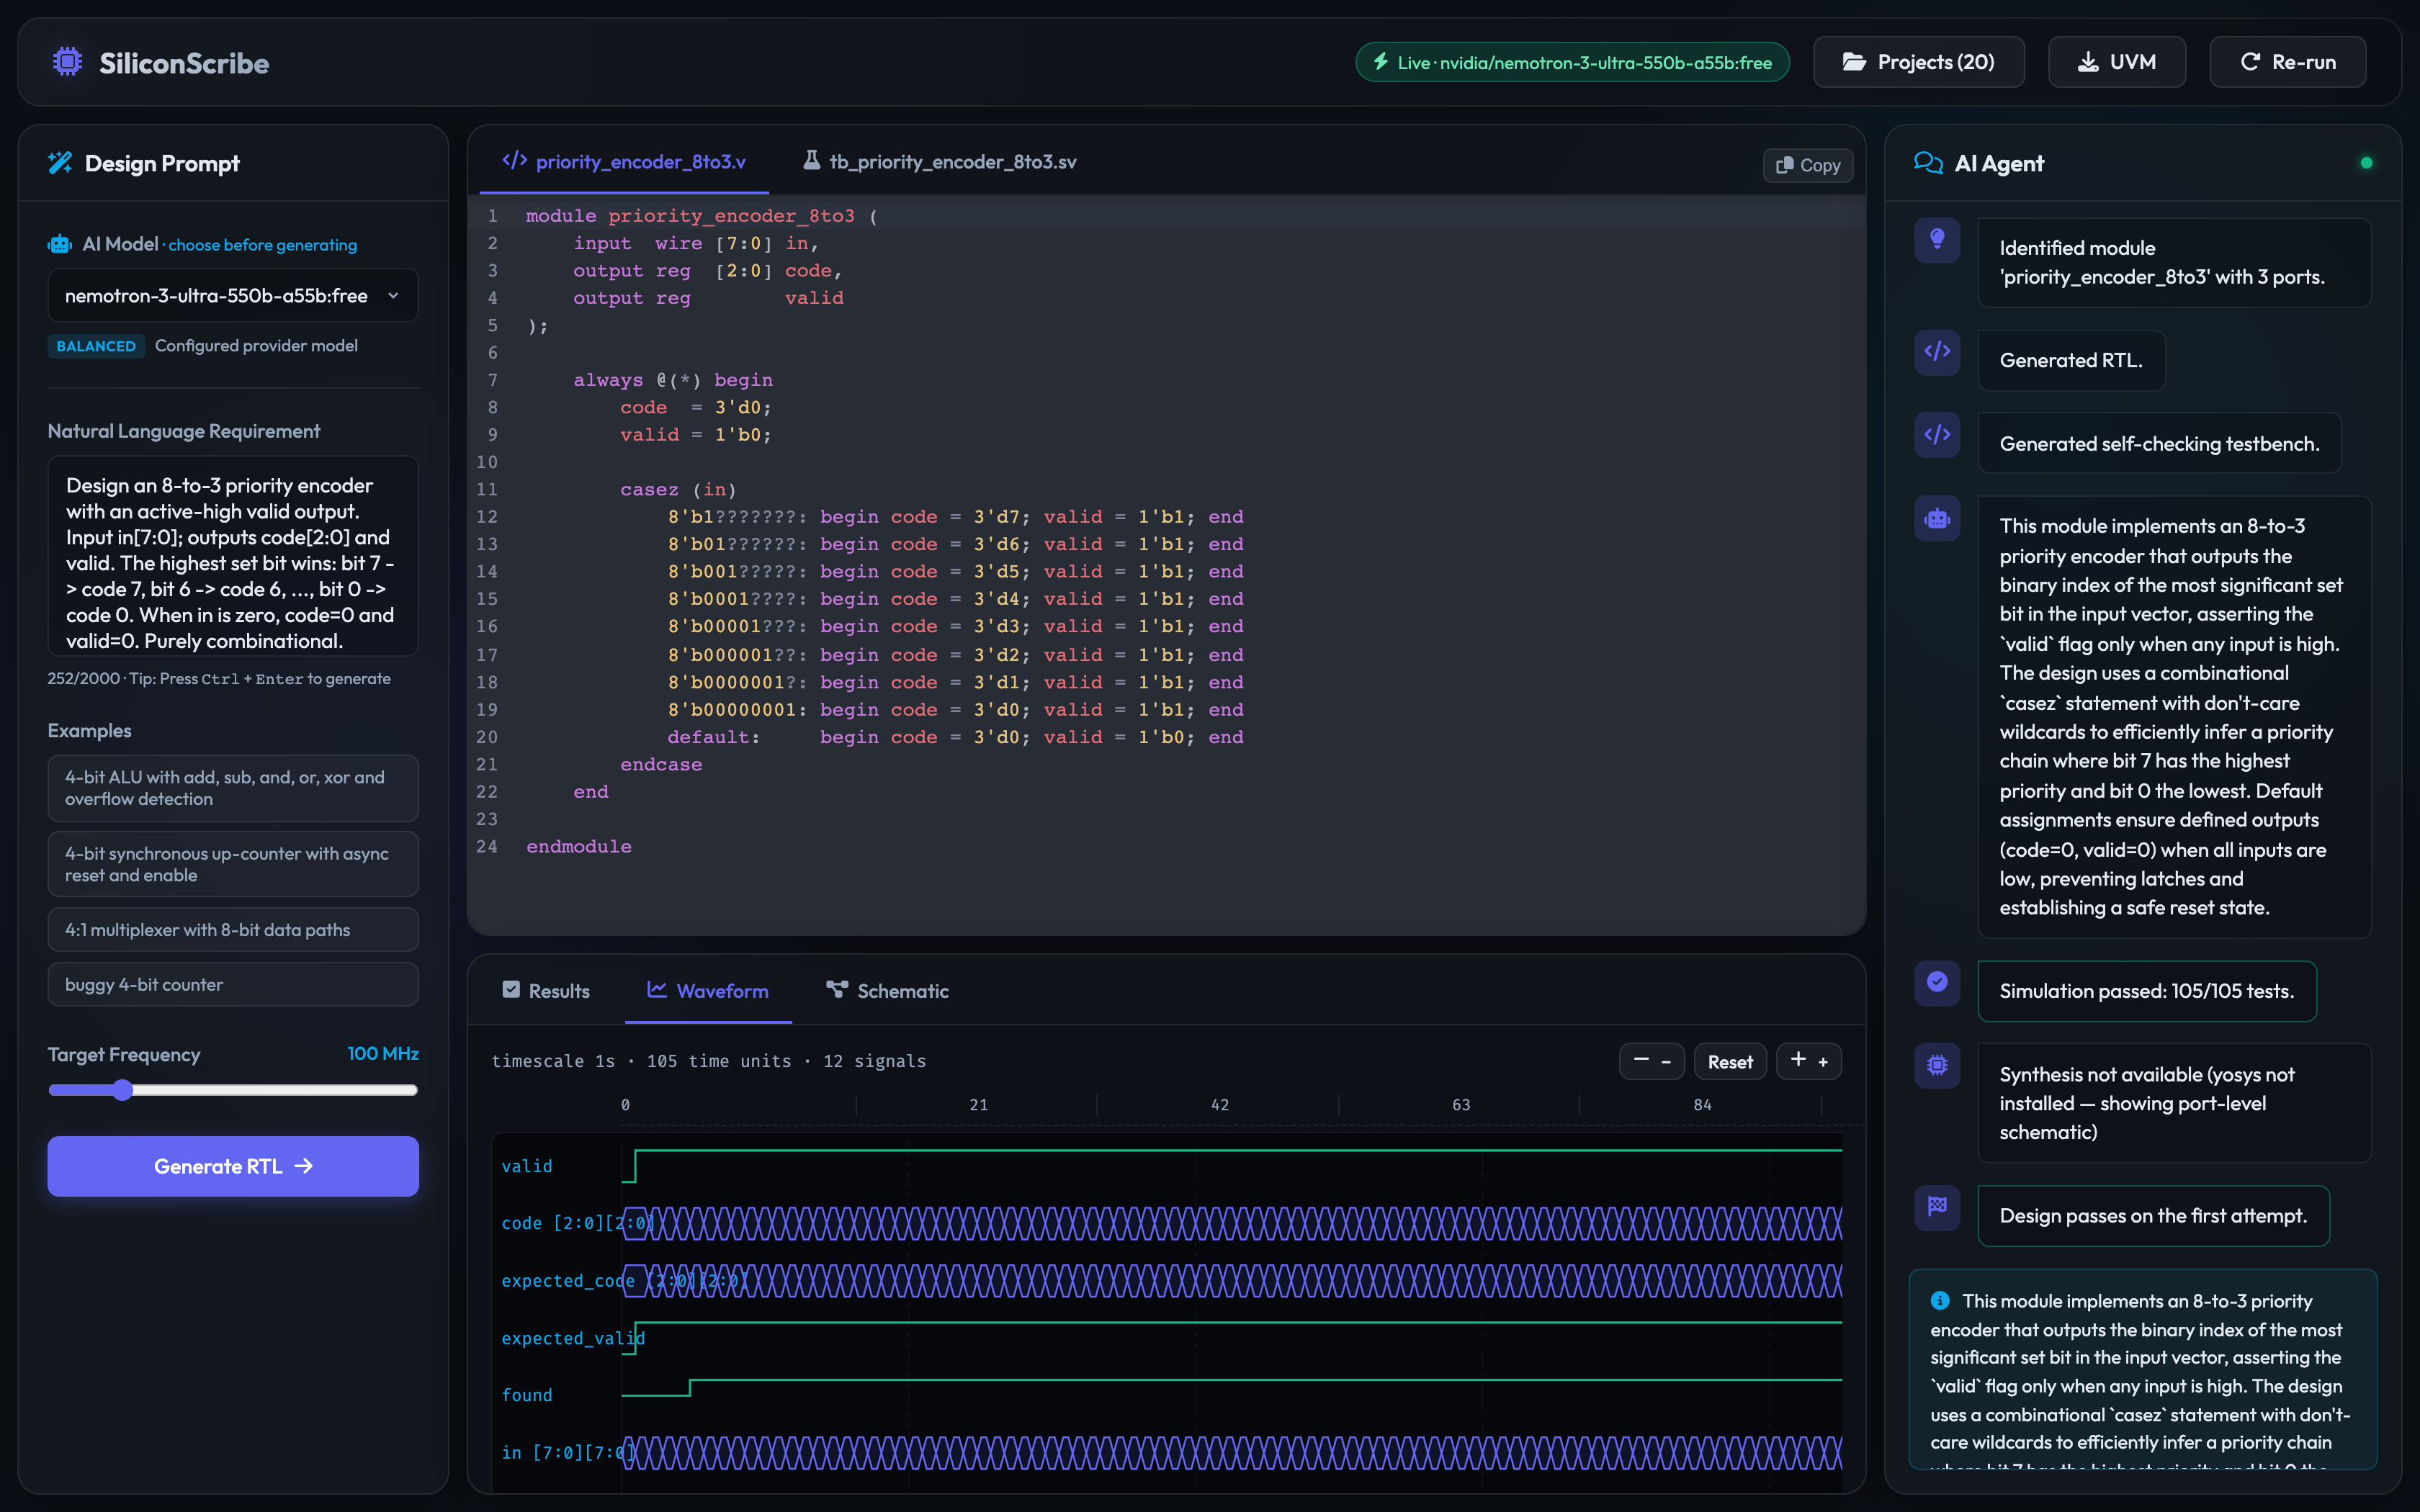
\includegraphics[width=0.78\textwidth]{04_waveform.png}
\caption{In-browser SVG waveform for the live run, parsed from the simulator's VCD.
The input, code, and valid signals are visible with a time ruler and hex bus
labels.}
\label{fig:wave}
\end{figure}

\begin{figure}[H]
\centering
\begin{minipage}[t]{0.34\textwidth}
\vspace{0pt}
\centering
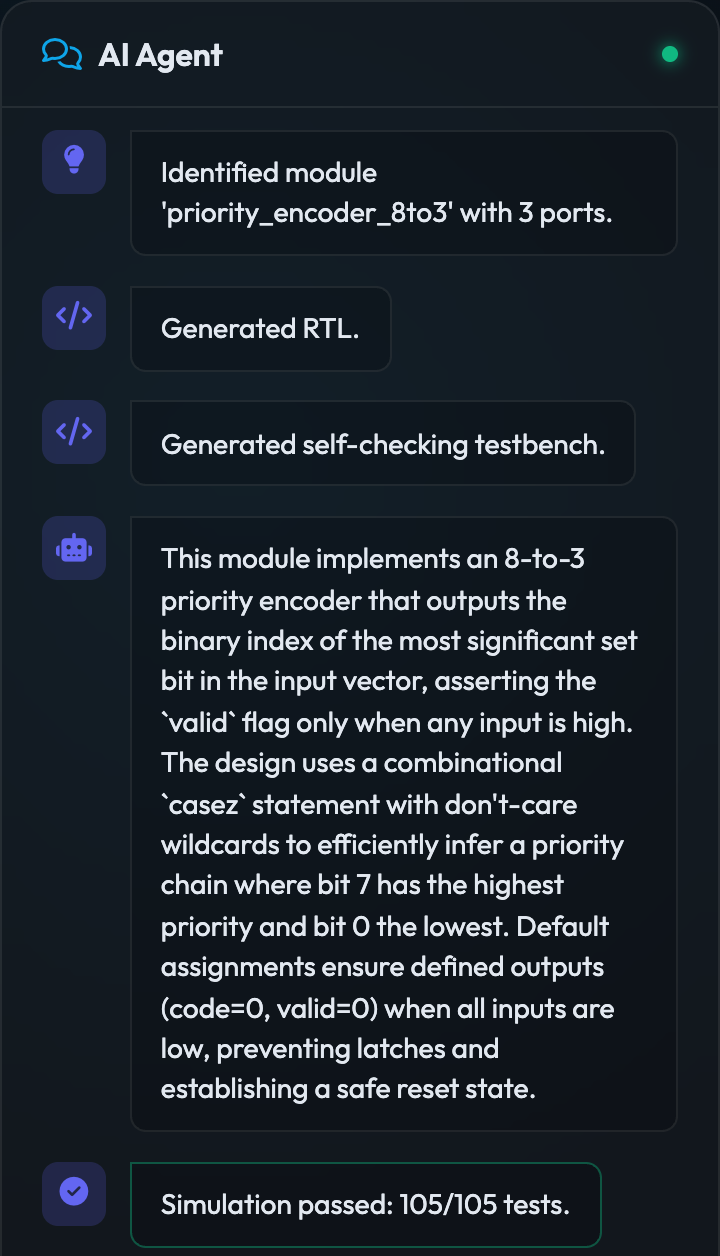
\includegraphics[width=\linewidth]{06a_agent_trace_top.png}
\end{minipage}\hfill
\begin{minipage}[t]{0.34\textwidth}
\vspace{0pt}
\centering
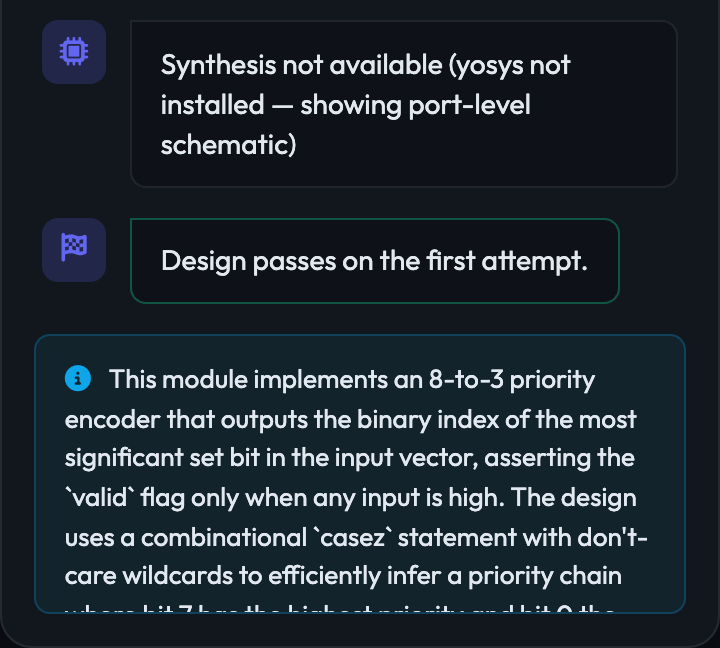
\includegraphics[width=\linewidth]{06b_agent_trace_bottom.png}\par
\vspace{3mm}
\raggedright\footnotesize
\textbf{Result summary}\par\vspace{1pt}
{\ttfamily\scriptsize Passed: 105\par Failed: 0\par Verdict: PASS\par}
\vspace{2.5mm}
\textbf{Live run facts}\par\vspace{1pt}
{\scriptsize
\begin{tabular}{@{}l@{\hspace{1.2em}}l@{}}
Model & {\tiny\texttt{nvidia/\allowbreak nemotron-3-ultra-550b-a55b:free}}\\
Iterations & 0\\
Fallback & none\\
\end{tabular}}
\end{minipage}
\caption{Agent timeline for the live run, split into two columns (left: intent, RTL,
independent testbench, explanation, and the simulator's ``105/105'' result; right:
synthesis note, final verdict, and explanation). The same run is shown in
Figure~\ref{fig:pass}.}
\label{fig:trace}
\end{figure}

\subsection{Live Fault Diagnosis and Repair}
Passing a correct design is necessary but not sufficient. The diagnostic path was
validated by injecting a known semantic bug into a counter and running the
\emph{live} fixer with the \emph{independent} testbench. This is not the scripted
offline fix: the LLM received the RTL, the testbench, the specification, and the
simulator log, and returned a structured diagnosis.

\begin{table}[H]
\centering
\caption{Live fault-injection result (real LLM diagnosis, real simulator).}
\label{tab:seeded}
\small
\begin{tabularx}{\textwidth}{@{}l c c c X@{}}
\toprule
 & \textbf{Passed} & \textbf{Failed} & \textbf{Status} & \textbf{Action} \\
\midrule
Before & 1 & 19 & \textcolor{failred}{\textbf{FAIL}} & initial buggy RTL (\code{count + 2'd2}) \\
After  & 20 & 0 & \textcolor{passgreen}{\textbf{PASS}} & LLM diagnosis + RTL patch (\code{count + 1'b1}) \\
\bottomrule
\end{tabularx}
\end{table}

The fixer's diagnosis, quoted from the live response, was:

\begin{quote}
\footnotesize
\textbf{Symptom:} The testbench expects the counter to increment by 1 each cycle
(expected sequence: 1,2,3...), but the actual output increments by 2 (got sequence:
2,4,6...). The first failure is at expected=1, got=2.\\
\textbf{Root cause:} In the RTL, the counter increments by \code{2'd2} (i.e., 2)
when enable is asserted, but the specification requires a standard up-counter that
increments by 1.\\
\textbf{Fix location:} \code{counter.v} line 10 (the line
\code{count <= count + 2'd2;}).\\
\textbf{Confidence:} high.
\end{quote}

This is the behaviour the project is meant to demonstrate: the model identifies the
\emph{actual} wrong line from the first failing vector, not a generic
``counter is broken'' fallback. The testbench was not weakened; it was the same
independent testbench before and after the fix.

\subsection{Self-Correction in the Application}
Figure~\ref{fig:repairui} shows the loop as the user sees it, using the built-in ``buggy 4-bit counter'' demonstration. This capture uses the offline provider, so the repair is the labelled scripted regression path rather than an LLM diagnosis (the live LLM diagnosis is Table~\ref{tab:seeded}). The initial RTL fails 25 of 27 checks; the loop applies the repair and the re-simulation passes 27 of 27. The iteration timeline records every attempt, and for a scripted fix the interface states that no root-cause diagnosis was produced instead of inventing one (Figure~\ref{fig:repairtl}).

\begin{figure}[H]
\centering
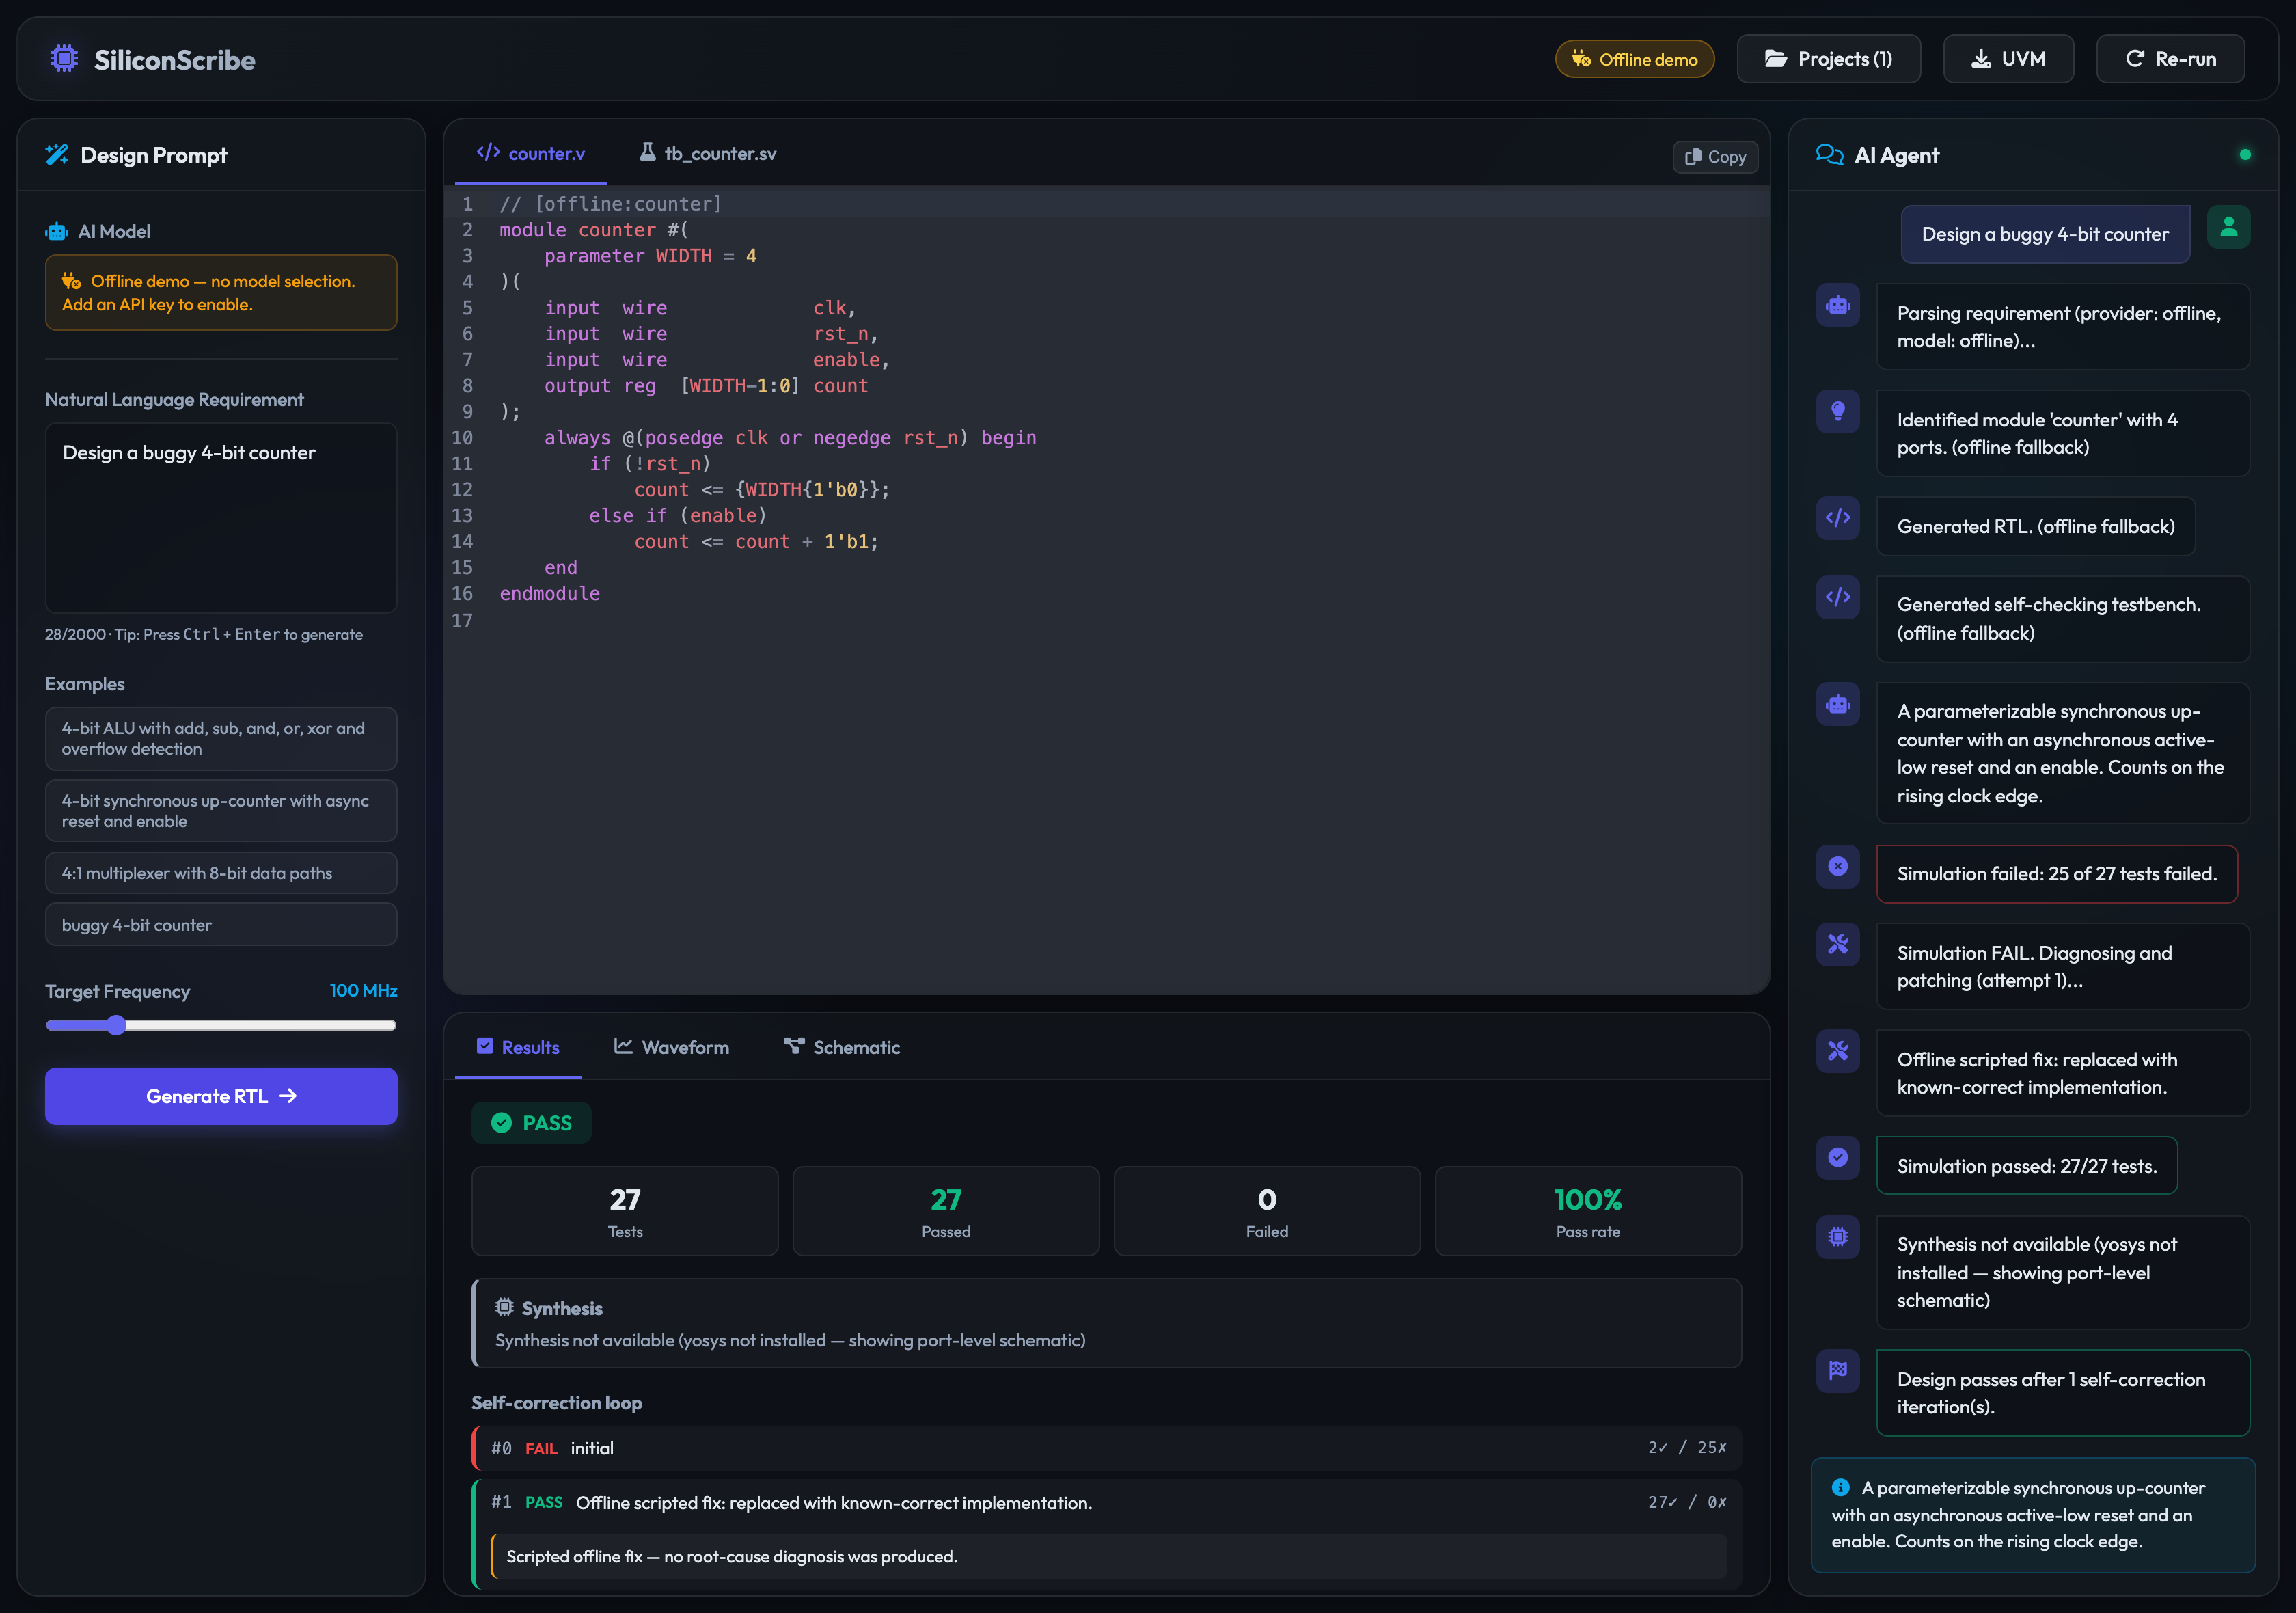
\includegraphics[width=0.60\textwidth]{07_repair_loop_ui.png}
\caption{Self-correction in the browser (offline demonstration path): the agent timeline shows the failing simulation, the repair step and the passing re-simulation, and the results panel shows the final PASS with the iteration history.}
\label{fig:repairui}
\end{figure}

\begin{figure}[H]
\centering
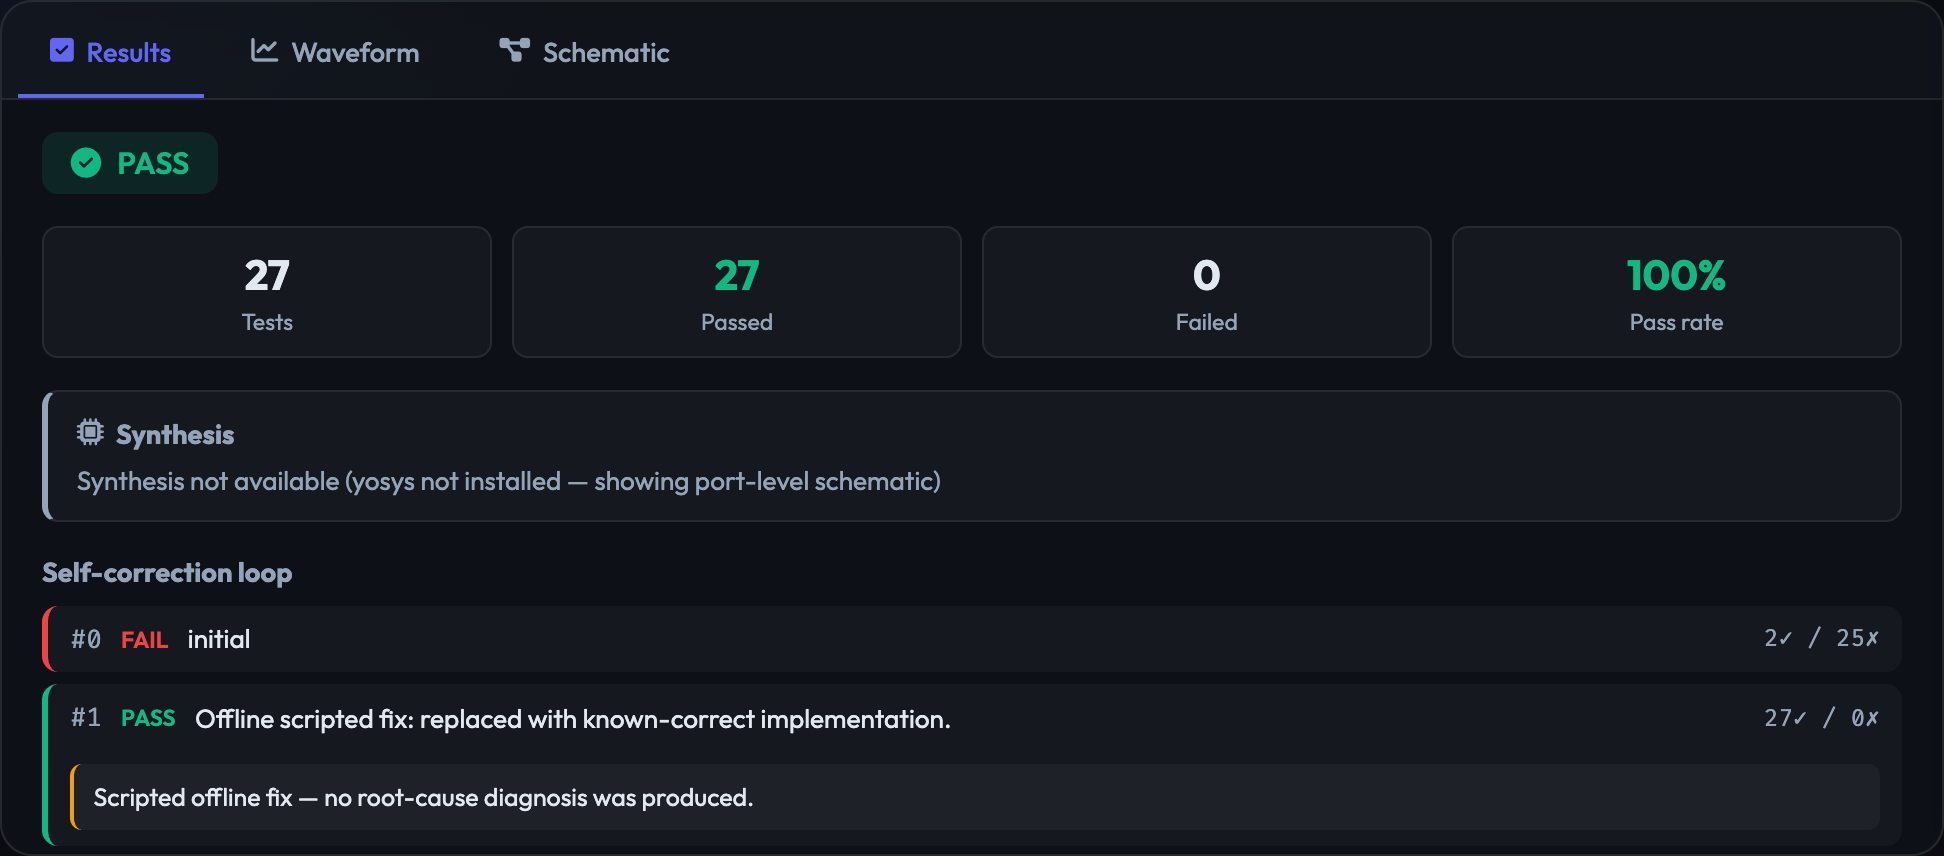
\includegraphics[width=0.8\textwidth]{08_repair_timeline.png}
\caption{Iteration timeline: attempt \#0 FAIL (2 passed / 25 failed), attempt \#1 PASS (27 / 0). The scripted fix is labelled and carries no fabricated diagnosis.}
\label{fig:repairtl}
\end{figure}

\subsection{Compiler-Repair Coverage}
Two mechanical repairs are covered by unit tests that run real Icarus:

\begin{itemize}
\item a testbench-level \code{wire} assigned in an \code{initial} block is changed
to \code{reg}, with a diagnosis naming \code{testbench.sv} and the signal;
\item a \code{disable <function>} early return is changed to
\code{return <function>}, preserving first-match semantics.
\end{itemize}

Both tests assert that the fixer LLM is \emph{not} called for a mechanical repair,
and that the subsequent simulation reaches PASS.

\subsection{Mutation Sweep: Can the Testbenches Fail?}
A testbench that passes everything is not evidence, so its strength was measured. One semantic bug at a time was injected into the golden RTL of each curated design and the curated testbench was required to turn PASS into FAIL. The first sweep killed 11 of 14 mutants; the three survivors were genuine testbench gaps: the counter testbench never turned \code{enable} off (so a counter that ignores \code{enable} passed), and the ALU testbench neither checked the \code{overflow} flag nor drove the undefined opcodes 5 to 7. The testbenches were then hardened (Table~\ref{tab:mutants}) and the sweep re-run.

\begin{table}[H]
\centering
\caption{Mutation sweep over the curated designs: first sweep versus after hardening the testbenches.}
\label{tab:mutants}
\small
\begin{tabular}{@{}l l c c@{}}
\toprule
\textbf{Design} & \textbf{Injected bug} & \textbf{First sweep} & \textbf{After hardening} \\
\midrule
counter & increment by 2 & \textcolor{passgreen}{killed} & \textcolor{passgreen}{killed} \\
counter & decrement & \textcolor{passgreen}{killed} & \textcolor{passgreen}{killed} \\
counter & reset polarity inverted & \textcolor{passgreen}{killed} & \textcolor{passgreen}{killed} \\
counter & reset ignored & \textcolor{passgreen}{killed} & \textcolor{passgreen}{killed} \\
counter & wrong reset value & \textcolor{passgreen}{killed} & \textcolor{passgreen}{killed} \\
counter & enable ignored & \textcolor{failred}{\textbf{survived}} & \textcolor{passgreen}{killed} \\
ALU & AND replaced by OR & \textcolor{passgreen}{killed} & \textcolor{passgreen}{killed} \\
ALU & ADD replaced by SUB & \textcolor{passgreen}{killed} & \textcolor{passgreen}{killed} \\
ALU & SUB replaced by ADD & \textcolor{passgreen}{killed} & \textcolor{passgreen}{killed} \\
ALU & XOR replaced by OR & \textcolor{passgreen}{killed} & \textcolor{passgreen}{killed} \\
ALU & overflow stuck at 0 & \textcolor{failred}{\textbf{survived}} & \textcolor{passgreen}{killed} \\
ALU & undefined opcode not zero & \textcolor{failred}{\textbf{survived}} & \textcolor{passgreen}{killed} \\
full adder & sum drops carry-in & \textcolor{passgreen}{killed} & \textcolor{passgreen}{killed} \\
mux4to1 & d0 and d1 swapped & \textcolor{passgreen}{killed} & \textcolor{passgreen}{killed} \\
\midrule
\multicolumn{2}{@{}l}{\textbf{Mutants killed}} & \textbf{11 / 14} & \textbf{14 / 14} \\
\bottomrule
\end{tabular}
\end{table}

The counter testbench gained an enable-hold phase, an asynchronous-reset phase and a resume phase (27 checks in total; the original 20-check phase is unchanged, so the archived live evidence still reproduces). The ALU testbenches now drive all eight opcodes and check the carry or borrow output against an independent wide-addition reference. The sweep is reproducible with \code{python3 tools/mutation_sweep.py}, and the regression suite pins 16 mutants. Figure~\ref{fig:hardtb} shows the hardened counter testbench in the editor and Figure~\ref{fig:alu} an ALU run against the hardened testbench.

\begin{figure}[H]
\centering
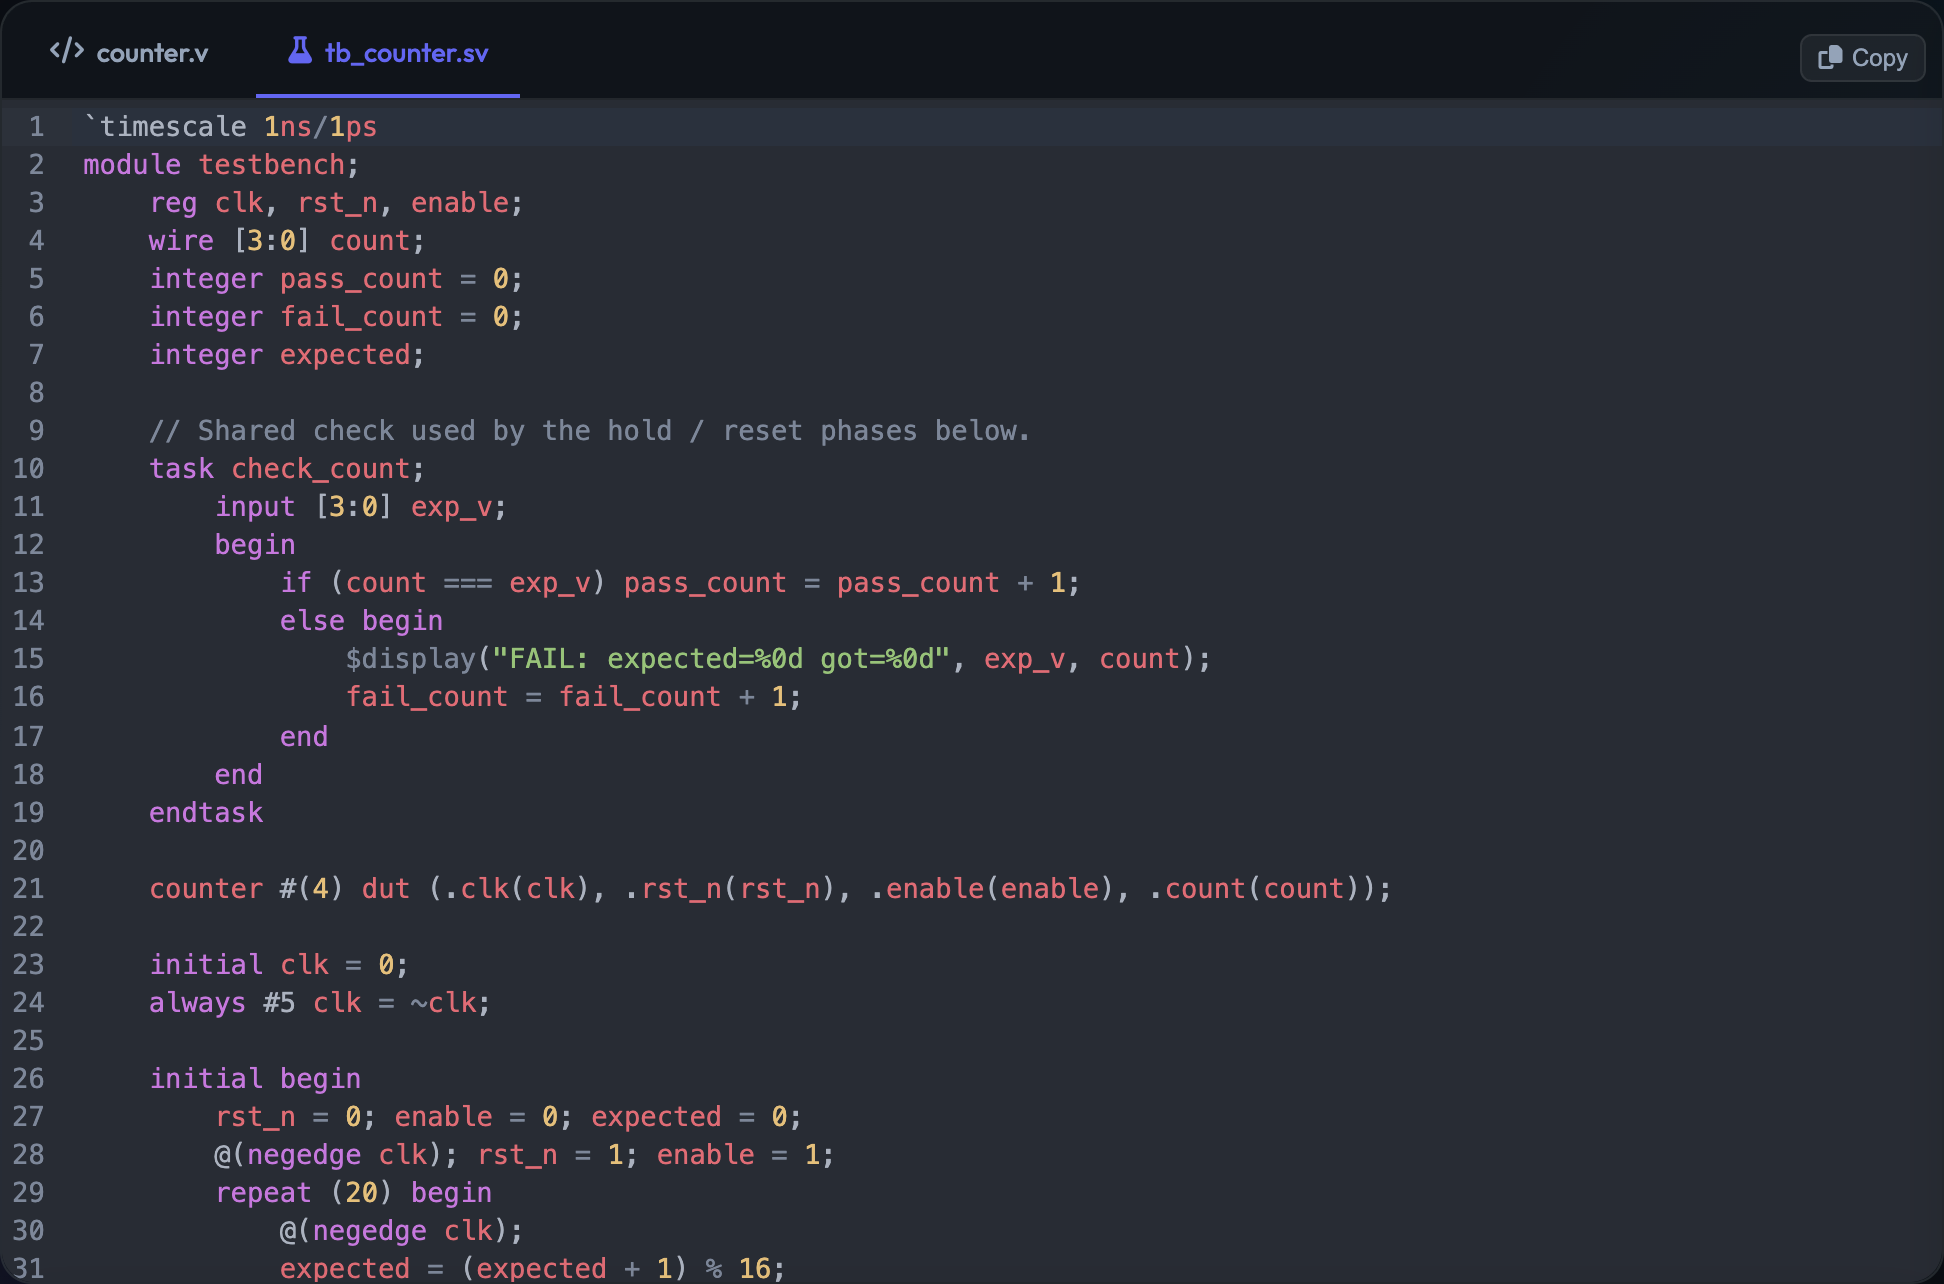
\includegraphics[width=0.58\textwidth]{11_hardened_testbench.png}
\caption{Hardened counter testbench (excerpt): a shared \texttt{check\_count} task is used by the new enable-hold, asynchronous-reset and resume phases.}
\label{fig:hardtb}
\end{figure}

\begin{figure}[H]
\centering
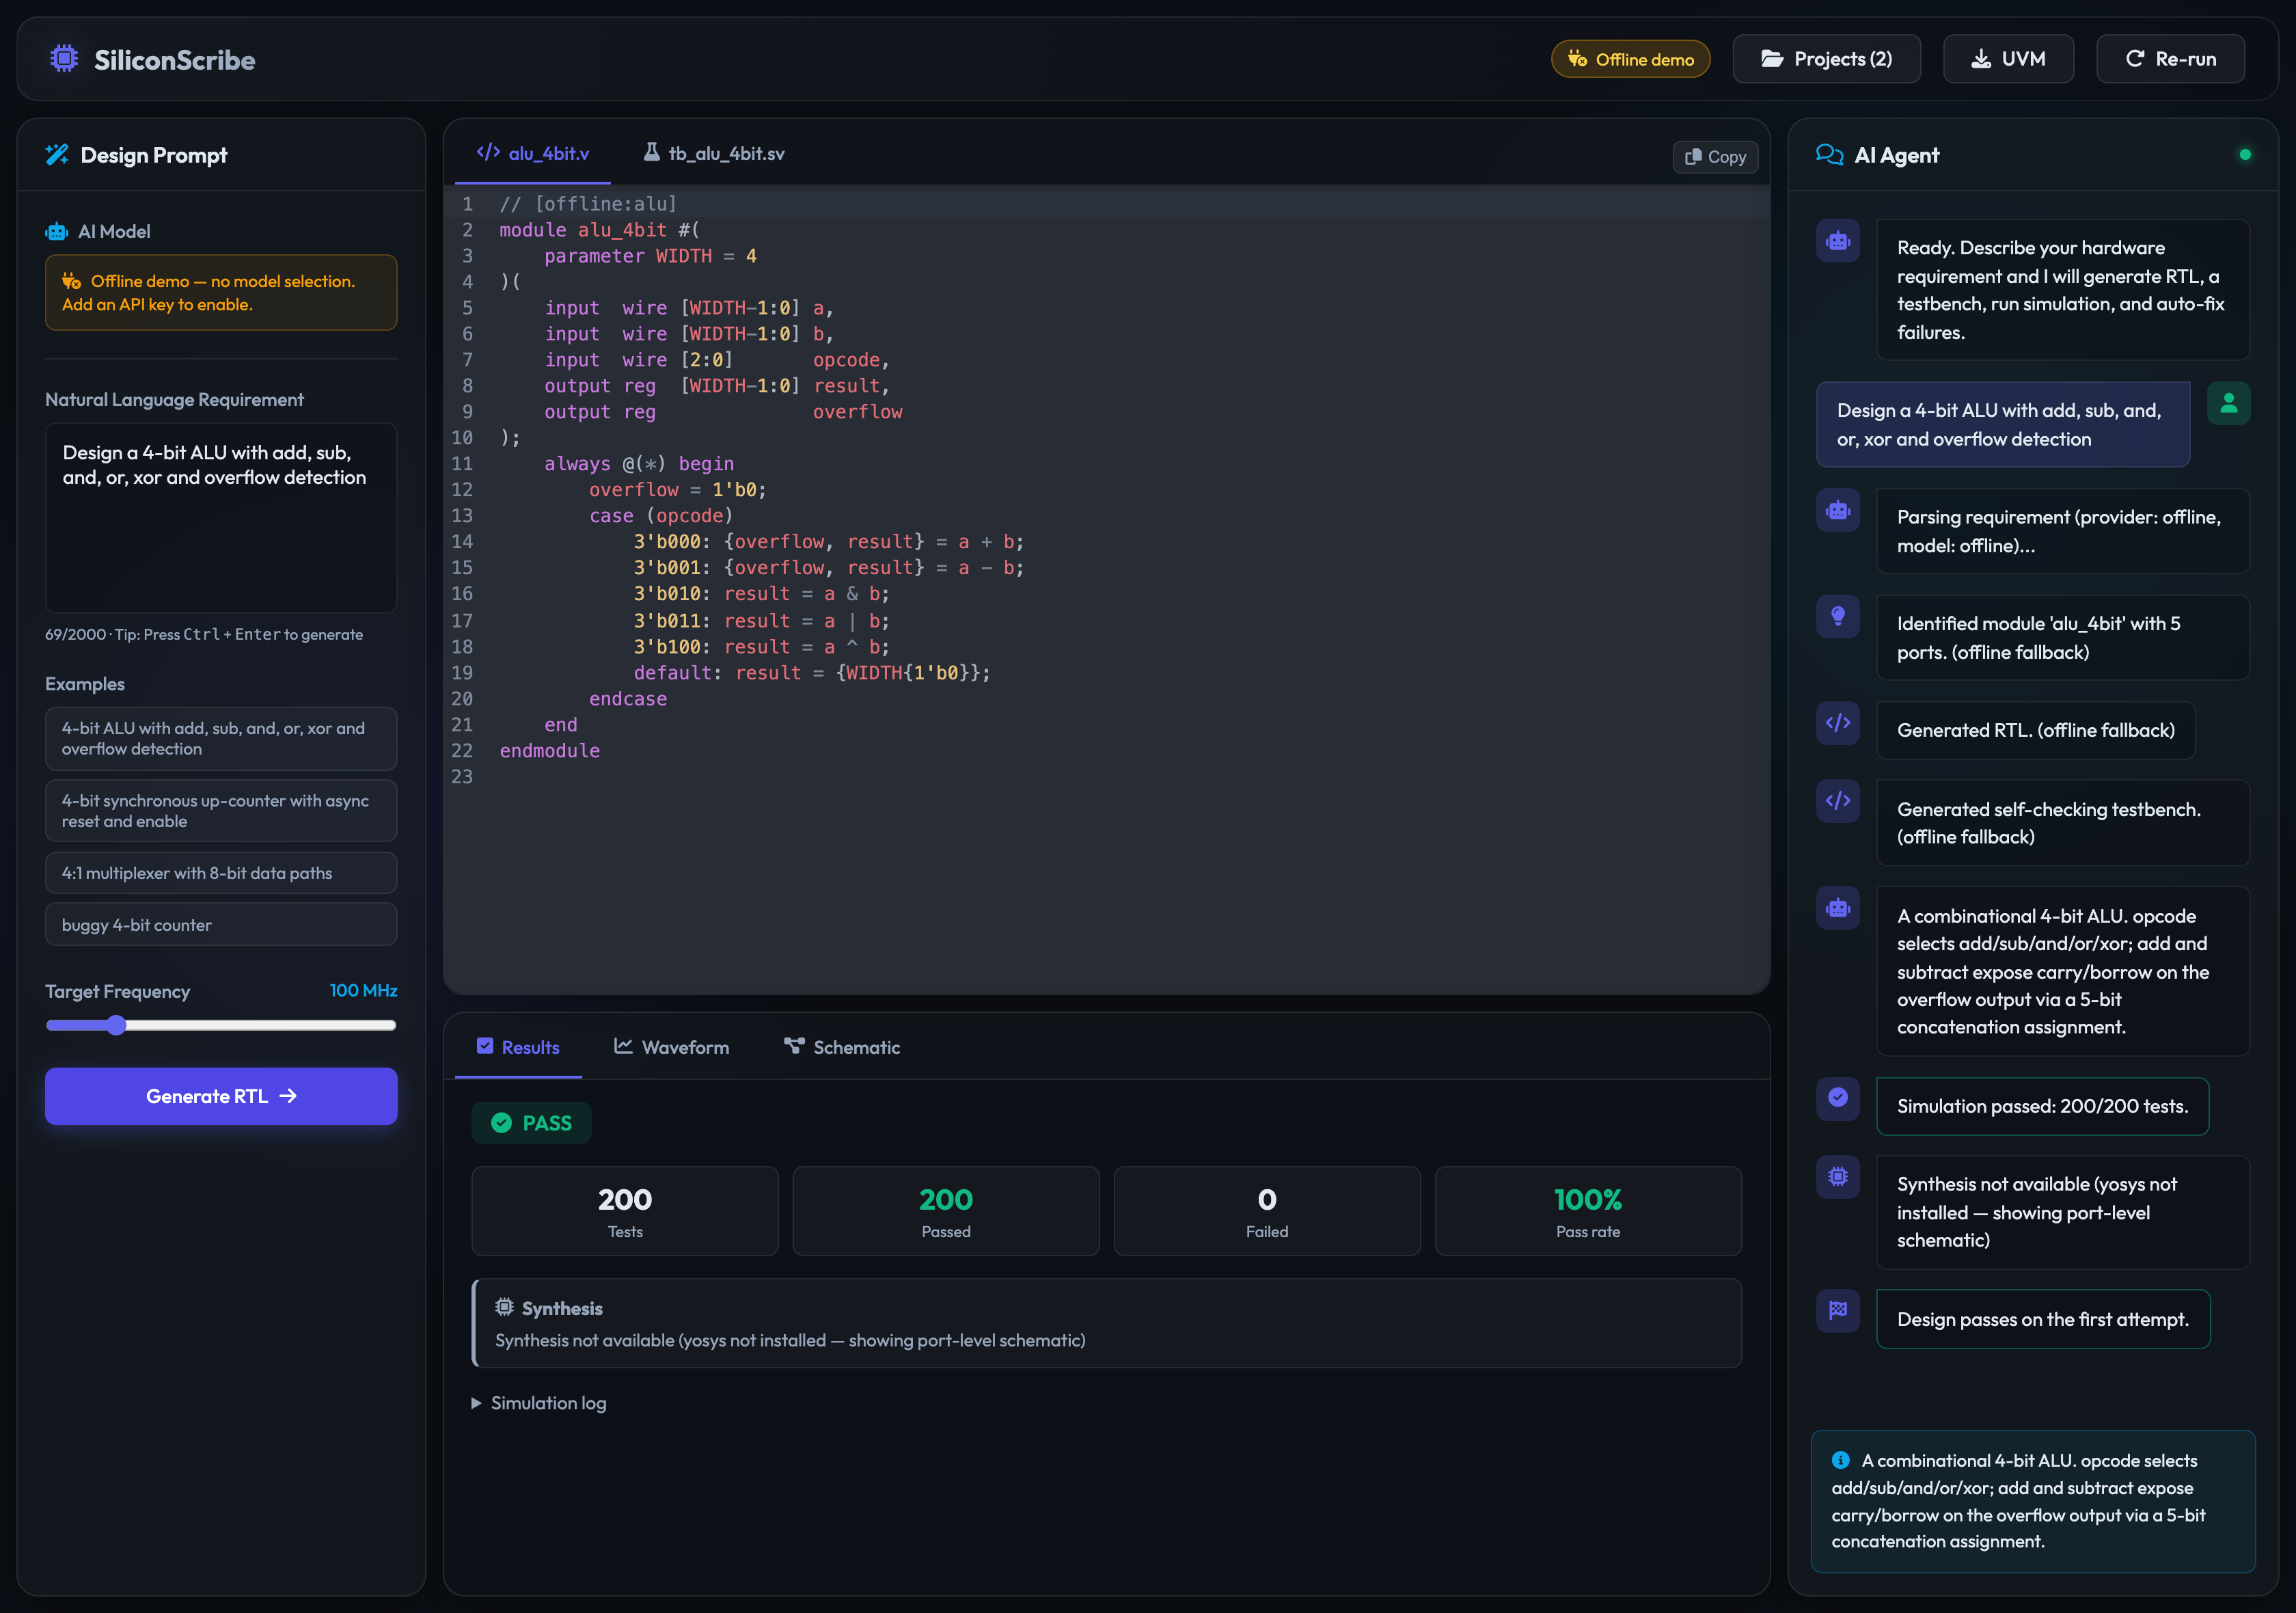
\includegraphics[width=0.60\textwidth]{14_alu_pass_hardened_tb.png}
\caption{ALU example run against the hardened testbench (200 checks covering all eight opcodes and the overflow output).}
\label{fig:alu}
\end{figure}

\subsection{Supporting Outputs}
The application also produces a port-level schematic, a three-tier lint report,
optional Yosys generic-cell counts when Yosys is installed, a bounded VCD waveform,
and a 16-file UVM 1.2 export. The final environment did not have Yosys installed;
the UI correctly reported ``Synthesis not available'' rather than fabricating area
numbers (visible in Figure~\ref{fig:pass}).

\subsection{Sequential Waveform and Schematic View}
Figure~\ref{fig:cwave} shows the waveform of a sequential design: the counter wraps from \code{0xf} to \code{0x0} and holds when \code{enable} drops, which is exactly the behaviour the hardened testbench now checks, and the testbench's own \code{expected}, \code{pass_count} and \code{fail_count} variables are visible alongside the DUT signals. Figure~\ref{fig:schem} shows the schematic tab, which is a port-level block diagram; a gate-level view needs Yosys netlist output and is listed as future work rather than implied.

\begin{figure}[H]
\centering
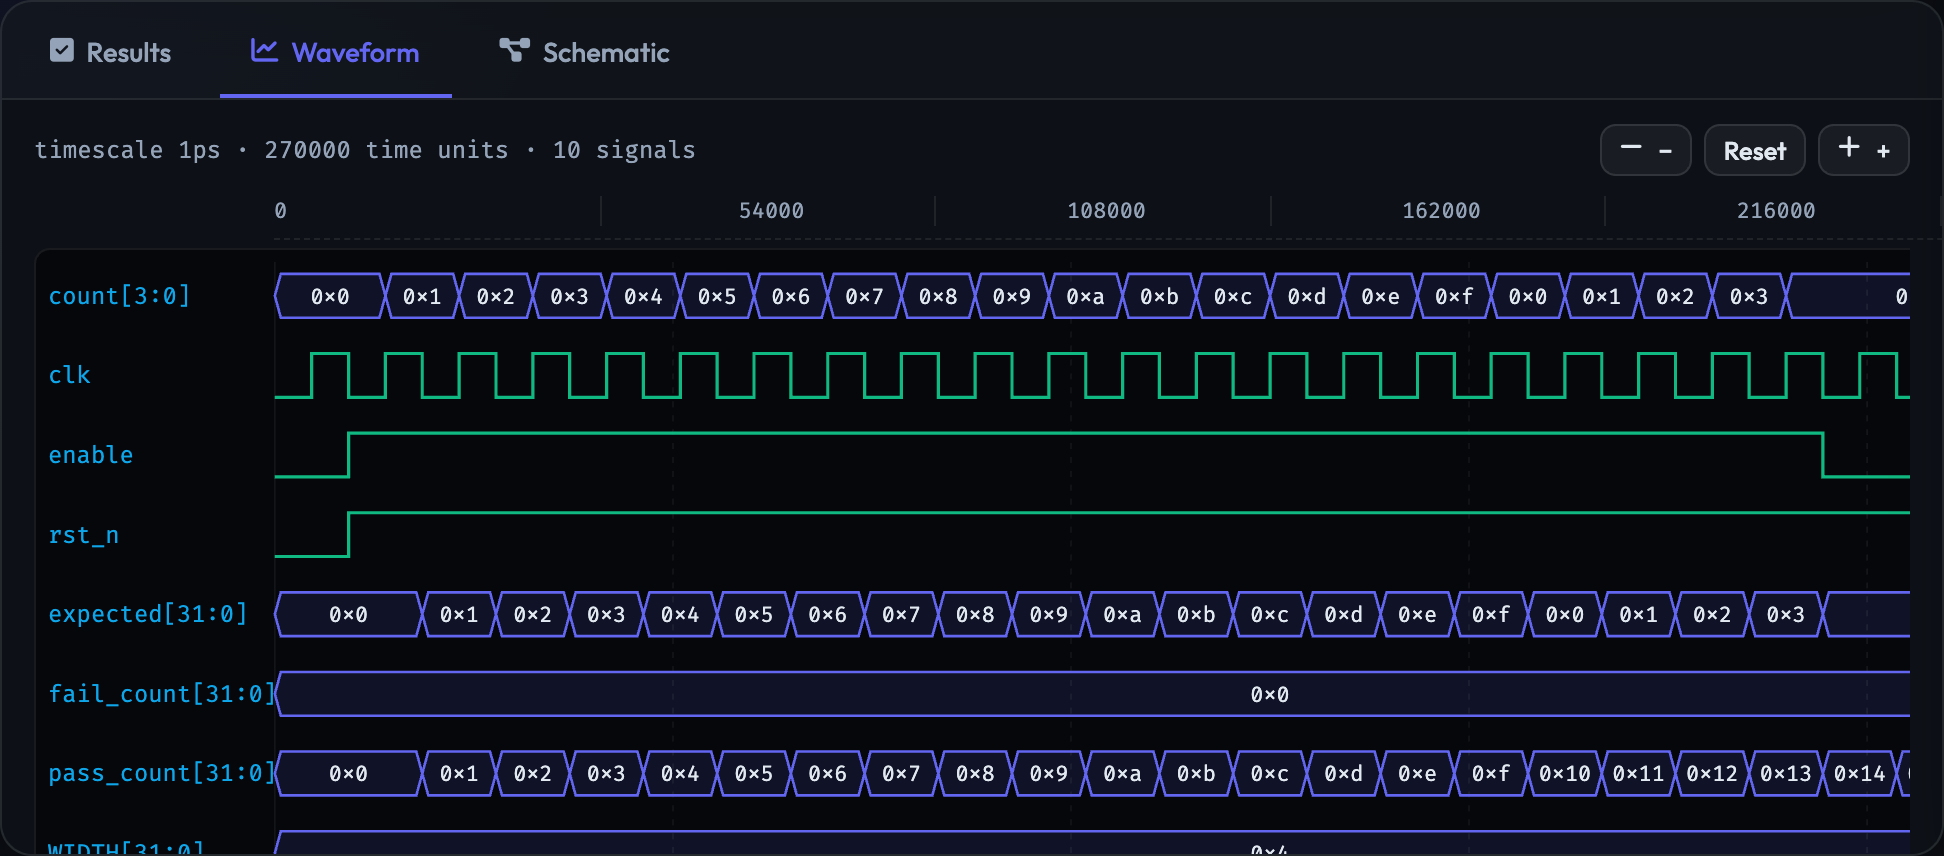
\includegraphics[width=0.8\textwidth]{09_counter_waveform.png}
\caption{Waveform of the counter parsed from the simulator's VCD: count wraps and holds when enable drops; the testbench's expected value and counters are visible.}
\label{fig:cwave}
\end{figure}

\begin{figure}[H]
\centering
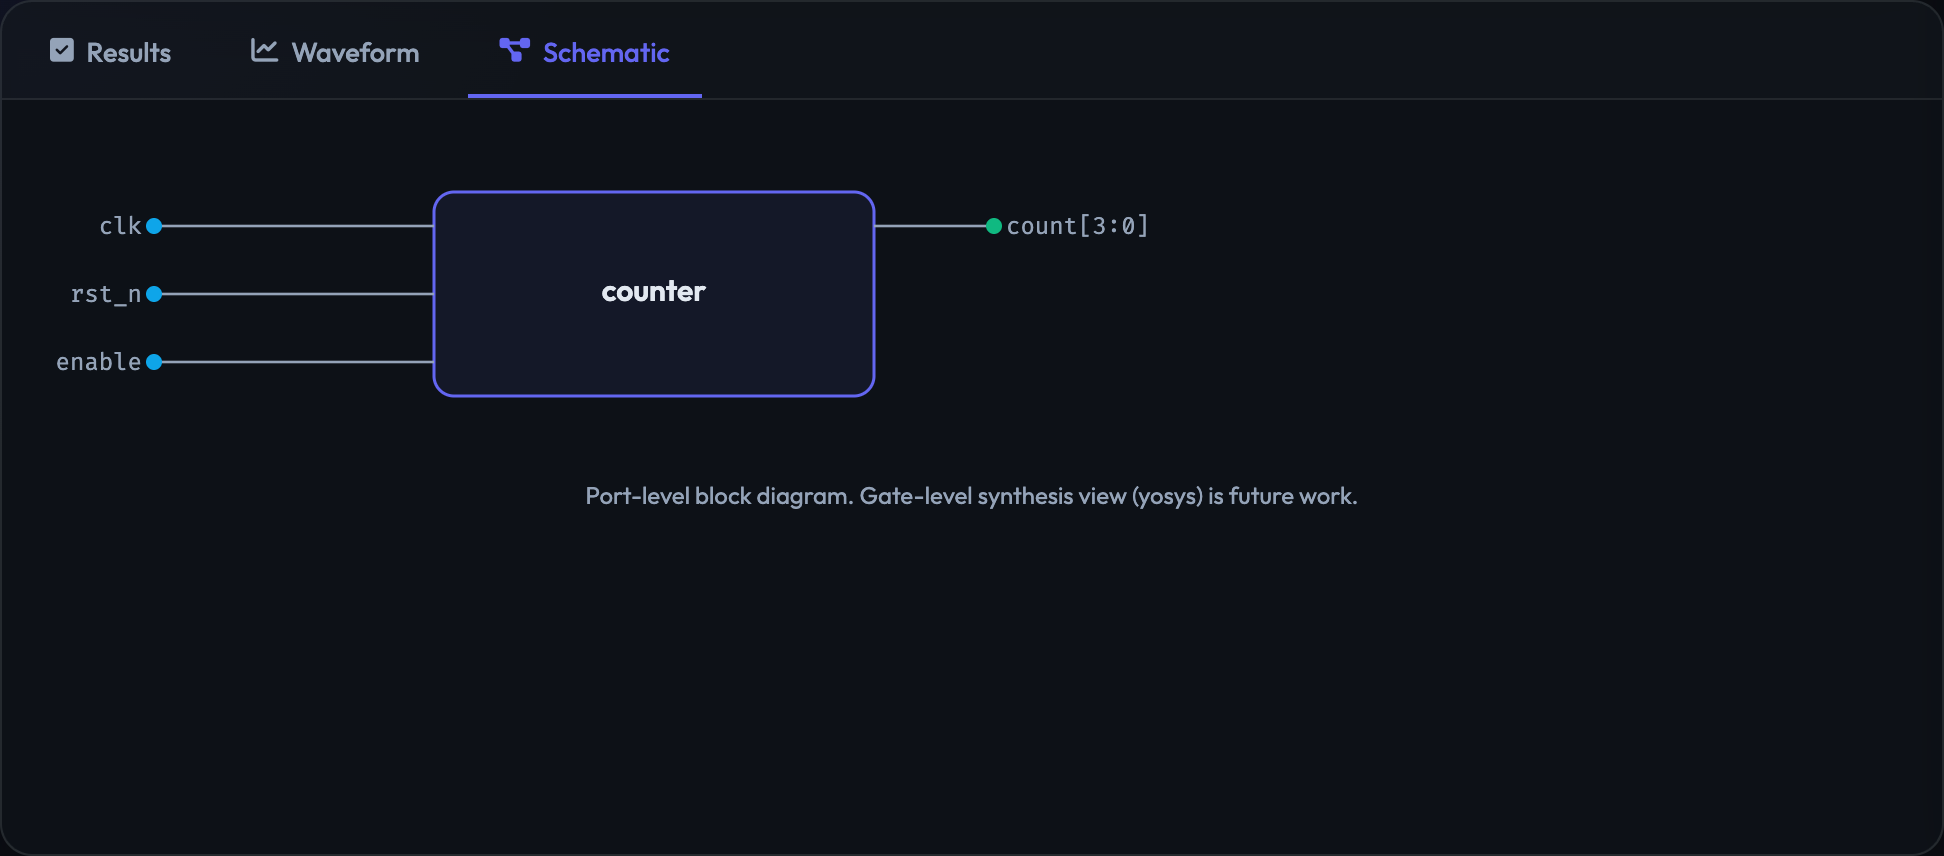
\includegraphics[width=0.7\textwidth]{10_schematic_view.png}
\caption{Schematic tab: port-level block diagram of the counter. The interface states that a gate-level view is future work.}
\label{fig:schem}
\end{figure}

\subsection{Project Persistence}
Finished runs are stored in SQLite and listed in the Recent Projects drawer with Load and Delete actions (Figure~\ref{fig:projects}). The final review found that only the blocking route saved a project while the browser uses the streaming route, so nothing generated in the interface ever appeared in the drawer. The streaming route now persists the finished run, and a regression test pins it.

\begin{figure}[H]
\centering
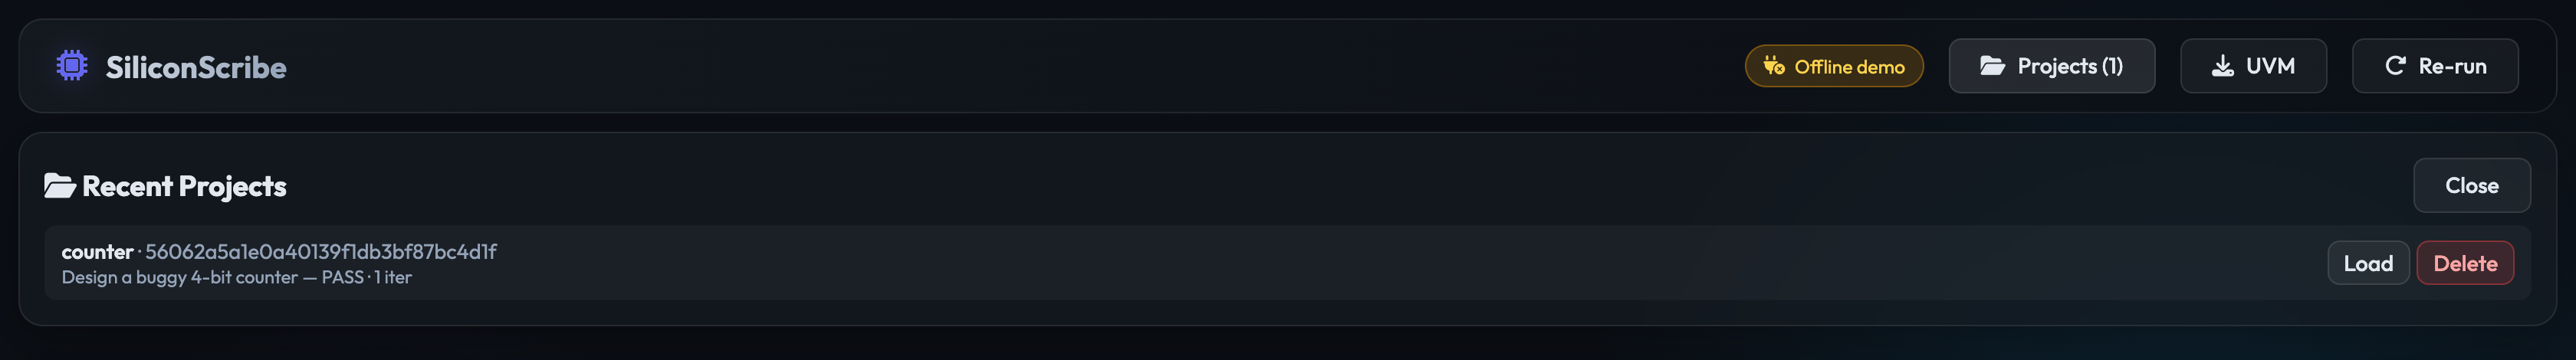
\includegraphics[width=\textwidth]{13_projects_drawer.png}
\caption{Recent Projects drawer listing a run that was generated through the streaming interface, with Load and Delete actions.}
\label{fig:projects}
\end{figure}

\subsection{Degraded Mode in the Application}
When a prompt matches no curated design in offline mode, the interface shows a degraded-mode banner instead of passing a representative counter off as the requested design (Figure~\ref{fig:degraded}). A UART-transmitter prompt, which no curated design implements, triggers it.

\begin{figure}[H]
\centering
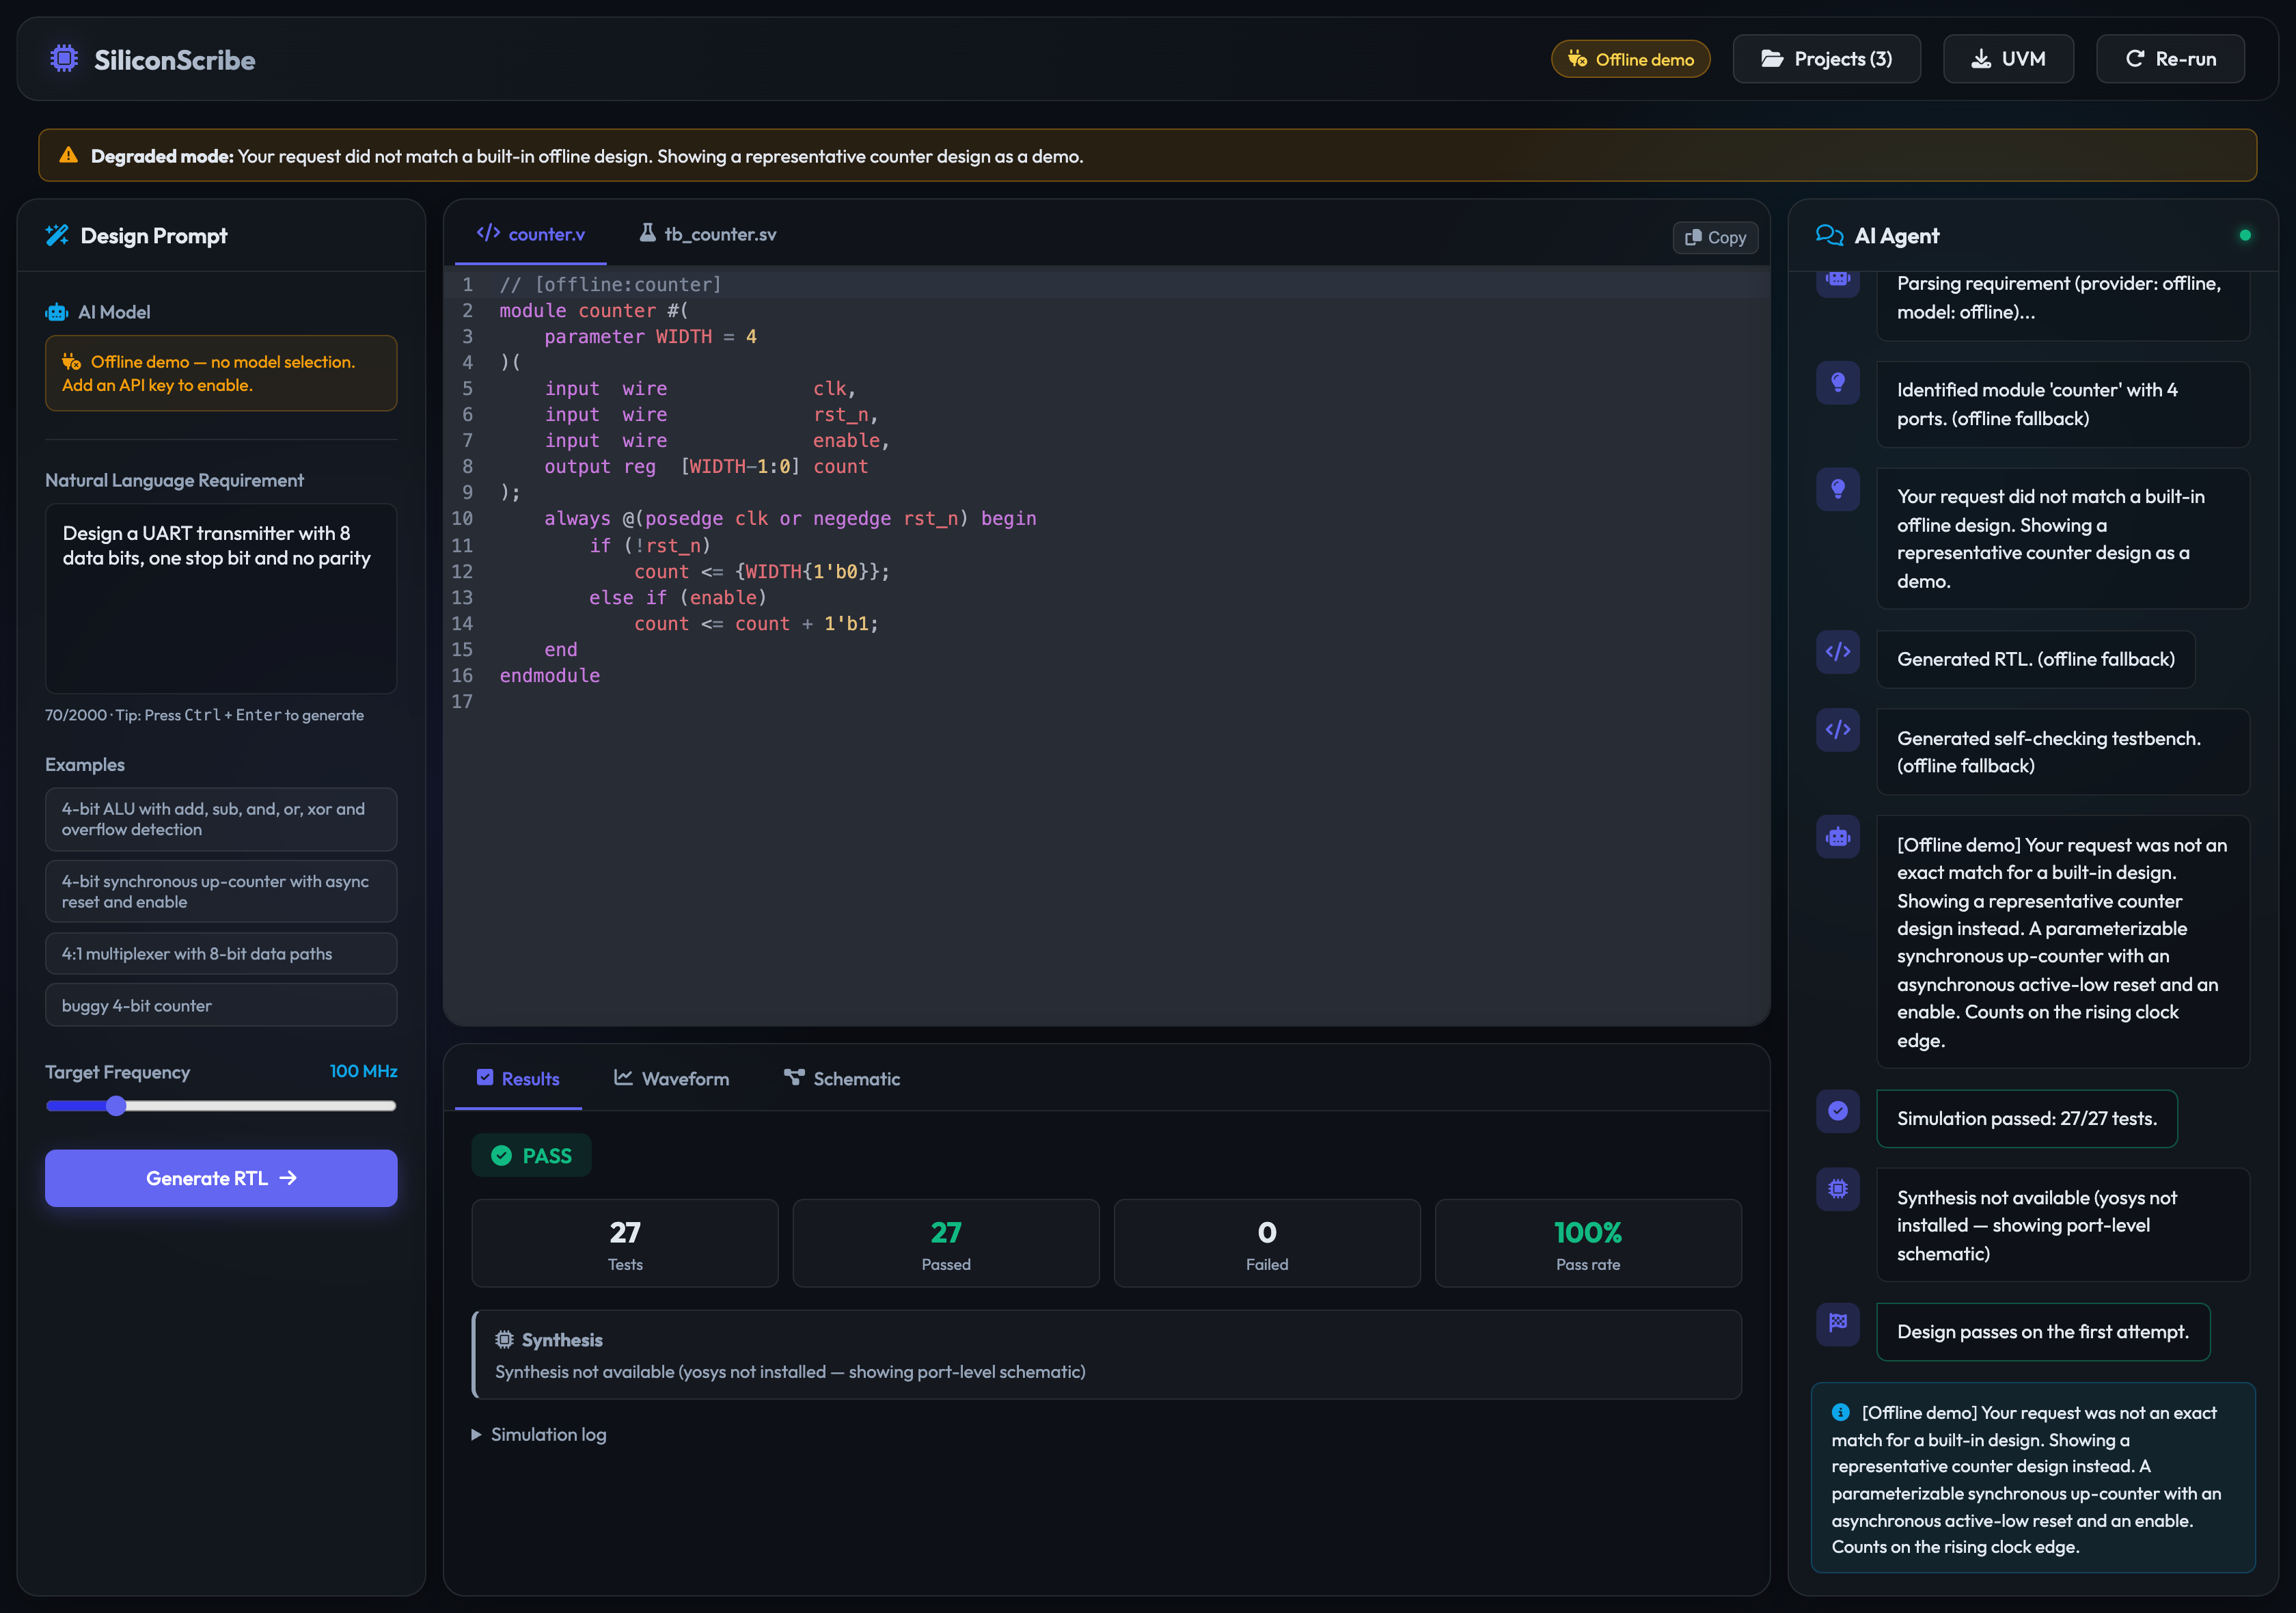
\includegraphics[width=0.60\textwidth]{12_degraded_mode.png}
\caption{Degraded-mode banner for a prompt that matches no built-in design (UART transmitter). The run is labelled as a demonstration instead of being presented as a UART.}
\label{fig:degraded}
\end{figure}

\subsection{Final Security and Robustness Review}
\label{sec:review}
Before submission the system was probed the way an examiner or attacker might, using executable probes against the running API rather than code reading alone. Table~\ref{tab:review} lists the findings and their measured before/after behaviour. One suspected path was refuted: command execution through \code{$system()} does not work on Icarus Verilog 12.0, which reports the task as undefined; the sandbox policy still rejects it because other simulator builds define it.

\begin{table}[H]
\centering
\caption{Findings of the final review and their measured effect.}
\label{tab:review}
\footnotesize
\begin{tabularx}{\textwidth}{@{}p{3.1cm}p{3.7cm}p{3.2cm}X@{}}
\toprule
\textbf{Finding} & \textbf{Probe} & \textbf{Before} & \textbf{After} \\
\midrule
Testbench could read and write arbitrary files & planted secret file plus file-I/O tasks sent to the simulation endpoint & secret returned in the API response; file written outside the workspace & rejected by the sandbox policy; nothing leaked or written; 18 regression tests \\
One run froze the server & health check while an 8~s simulation runs & 6.5~s & 1~ms (blocking routes run in a thread pool; rate limiter locked) \\
Weak testbenches & 14-mutant sweep & 11 of 14 killed & 14 of 14 killed \\
Browser runs never saved & generate in the UI, open the drawer & not listed & listed; regression test \\
Tests wrote to the real database & row count before and after the suite & grew on every run & unchanged (isolated workspace) \\
Duplicated interface text & screenshots & bit range printed twice on waveform labels; degraded notice shown twice & each shown once \\
\bottomrule
\end{tabularx}
\end{table}

% ========================================================== 6. DISCUSSION =
\section{Engineering Findings}
\label{sec:discussion}

The final system is the product of several live failures. They are reported here
because they are the most transferable part of the work.

\begin{table}[H]
\centering
\caption{Live failure modes found during validation and their fixes.}
\label{tab:failures}
\footnotesize
\begin{tabularx}{\textwidth}{@{}p{3.9cm}p{5.3cm}X@{}}
\toprule
\textbf{Failure} & \textbf{Evidence} & \textbf{Fix} \\
\midrule
Reasoning tokens consumed the output budget & Empty \code{content}; the model's scratchpad was almost used as a testbench & Reasoning disabled by default; empty-content error is explicit; reasoning text is never returned as code \\
Silent mid-run offline swap & A live run failed at intent parsing and was replaced by a curated design & Disable fallback after the first successful live call; fail honestly \\
wire assigned in a procedural block & Icarus: ``not a valid l-value'' & Deterministic wire$\rightarrow$reg repair, scoped by file \\
\code{disable} inside a function & Icarus: ``cannot disable functions'' & Deterministic \code{disable}$\rightarrow$\code{return} repair \\
Testbench oracle width bug & 35-bit concatenation compared with a 4-bit output; expected and got printed identically & Prompt requires width-correct comparisons; fixer checks the oracle against the spec \\
Malformed JSON fix response & Unescaped Verilog quotes/newlines broke the parser & XML-section protocol plus tolerant JSON salvage \\
Model listing mismatch & UI offered a Zen model while OpenRouter was active; the run fell back & \code{/api/models} exposes only the configured model when it is not curated \\
TB-only fix discarded & The loop hashed only the RTL, so an oracle repair looked like a no-op & State hash covers RTL \emph{and} TB \\
\bottomrule
\end{tabularx}
\end{table}

Two conclusions follow. First, \textbf{the model is not the only source of bugs}:
the orchestrator, the prompt contract, the response parser, and the model catalog
all produced defects that looked like ``the LLM is weak.'' Second, \textbf{the
simulator is the right oracle}: every one of these defects was found by executing
the pipeline, not by reading the code.

Model choice also matters. The free Nemotron Lightning model produced plausible but
incorrect Boolean equations for the priority encoder; the larger
\code{nvidia/nemotron-3-ultra-550b-a55b:free} produced a correct \code{casez} chain
that passed the independent specification-derived testbench. The application therefore reports
the active model and does not pretend all models are equivalent.

% ========================================================== 7. SCALE ======
\section{Scalability and Extensibility}
\label{sec:scale}

SiliconScribe was built model-agnostic and tool-agnostic. Every result in this report was obtained with free-tier language models because of budget, not because of an architectural limit: the provider is an OpenAI-compatible endpoint selected by three environment variables, so a stronger model is a configuration change, not a code change.

\subsection{Quality scales with the model}
The project already contains a measured example. On the same priority-encoder prompt, the free Nemotron Lightning model produced plausible but incorrect Boolean equations, while the larger \code{nvidia/nemotron-3-ultra-550b-a55b:free} model produced a correct \code{casez} chain that passed the independent specification-derived testbench on the first attempt (Section~\ref{sec:discussion}). The same pipeline and the same simulator judged both outputs, and the simulator exposed the first model's error rather than the model's own claim. The expected effect of a frontier or domain-tuned model is therefore a higher first-attempt pass rate and fewer repair iterations, with the simulator still deciding PASS or FAIL.

\subsection{Per-stage model routing}
The pipeline already separates five model calls: specification parsing, RTL generation, testbench generation, explanation and diagnosis-and-repair. A deployment can route each to a different model with \code{LLM_MODEL_INTENT}, \code{LLM_MODEL_RTL}, \code{LLM_MODEL_TESTBENCH}, \code{LLM_MODEL_EXPLAIN} and \code{LLM_MODEL_FIX}. The sensible policy is to spend budget where correctness is decided, a strong model for the testbench and the diagnosis, and a cheap model for the cosmetic explanation. A model chosen explicitly per request still takes precedence, and the web interface's default selection does not disable routing. This is implemented and covered by five automated tests.

\subsection{Scaling dimensions}
\begin{table}[H]
\centering
\caption{What is in place today and the path to scale along each dimension.}
\label{tab:scale}
\footnotesize
\begin{tabularx}{\textwidth}{@{}p{2.5cm}XX@{}}
\toprule
\textbf{Dimension} & \textbf{In place today} & \textbf{Scaling path} \\
\midrule
Language models & Any OpenAI-compatible endpoint (OpenRouter, Zen, NVIDIA NIM, OpenAI, self-hosted servers); per-request model and reasoning effort; model catalogue endpoint & Frontier and domain-tuned RTL models (for example VeriGen- or ChipNeMo-style) behind the same interface; automatic model selection driven by an evaluation suite \\
Stage routing & Five stage models by environment variable (implemented, tested) & Cost, latency and accuracy aware routing policy; fallback chains \\
Verification strength & Specification-only testbench; anti-cheat guard; measured mutation score & Two different models write independent testbenches and disagreement is flagged; golden reference models; SVA assertions; coverage-directed stimulus \\
Machine-learning models beyond LLMs & Clear seams: spec parsing, stimulus, diagnosis & Learned stimulus and coverage-closure agents; retrieval of similar verified designs as examples; learned bug localisers that rank suspicious RTL lines from failing vectors \\
EDA toolchain & Icarus Verilog; Yosys and Verilator hooks degrade gracefully; OpenROAD stub & Verilator coverage; Yosys with liberty files and OpenSTA for real area and timing; OpenROAD \\
Runtime & Single FastAPI process; blocking routes in a thread pool; SQLite; in-memory rate limiter & Job queue and worker pool; container or microVM sandbox per simulation; PostgreSQL; authentication and tenancy; object storage; metrics and tracing \\
Design size & Single blocks, roughly up to 1000 lines & Hierarchical decomposition: specification to sub-blocks to integration tests \\
\bottomrule
\end{tabularx}
\end{table}

\subsection{What this does and does not claim}
Scalability of \emph{model quality} is demonstrated above and the routing seam is implemented. Scalability of \emph{load}, many concurrent users, requires the runtime items in Table~\ref{tab:scale}: the current deployment is a single node with an in-process rate limiter and a local database. These are infrastructure additions around an unchanged core, not a redesign. With a modest budget the same code runs on stronger models; the constraint today is cost, not architecture.

% ========================================================== PROJECT ======
\section{Project Timeline, Deployment and Cost}
\label{sec:project}

\subsection{Development timeline}
\begin{table}[H]
\centering
\caption{Milestones (from the repository history and dated artefacts).}
\label{tab:timeline}
\footnotesize
\begin{tabularx}{\textwidth}{@{}p{2.6cm}X@{}}
\toprule
\textbf{Date (2026)} & \textbf{Milestone} \\
\midrule
23 July & Baseline; Docker, CI/CD, structured logging, health check, rate limiting, no-progress guard, VCD truncation metadata, frontend and backend tests \\
29 August & Zero-budget provider, hardening, lint and synthesis wrappers, SQLite projects, UVM export; QA and security audit \\
4--5 September & Vercel and Render free-tier deployment, live provider, 8-bit ALU, real reasoning-effort levels, CORS and rate-limit fixes \\
15 October & Progress report \\
September--November & Specification-only testbenches, structured diagnosis, compiler repairs, honest degraded mode, live validation \\
6 November & Live evidence captured; final review (sandbox, server freeze, testbench hardening, persistence fix, model routing); final report and presentation \\
\bottomrule
\end{tabularx}
\end{table}

\subsection{Deployment}
A multi-stage Docker image builds the frontend with Node 20 and serves it from a Python 3.12 image that also contains Icarus Verilog and Yosys, with a health check on \code{/health}. The configuration targets Vercel for the static frontend (which rewrites \code{/api} to the backend) and Render for the backend container; free tiers sleep when idle, so the interface explains cold-start delays. Docker Compose runs the whole system locally in one container.

\subsection{Cost}
Development and validation cost nothing beyond the laptop: open-source tools and free-tier models. When scaling, cost is driven by tokens per model call times calls per run, plus hosting. Per-stage routing keeps the expensive model on the testbench and diagnosis stages only, and the deterministic compiler repairs avoid model calls altogether for mechanical errors.

\subsection{Third-party components}
Icarus Verilog (GPL-2.0), Yosys (ISC), FastAPI and Pydantic (MIT), Uvicorn (BSD-3-Clause), React, Vite and CodeMirror (MIT) and SQLite (public domain). Generated designs belong to the user; no user data leaves the server except the prompt and code sent to the chosen model provider.

% ========================================================== 7. LIMITS =====
\section{Limitations}
\label{sec:limits}

\begin{enumerate}[label=\textbf{L\arabic*.},ref=L\arabic*]
\item \textbf{Residual common-mode model risk.} The testbench no longer sees the
RTL, which removes direct circularity, but the same model still interprets the
specification for both artifacts. If it misreads the specification identically in
both, the pair can still agree while being wrong. The specification parser is
therefore required to state reset polarity, opcode tables, and edge cases
explicitly; a future golden reference model would remove this risk.
\item \textbf{Single-block scope.} The pipeline targets single modules or small
blocks (roughly $\le 1000$ RTL lines). Multi-clock SoCs and hierarchical designs
exceed a single prompt.
\item \textbf{No static timing analysis or PPA sign-off.} The frequency hint is
textual. There is no SDC, no clock constraint, and no setup/hold analysis. Yosys,
when present, maps to its generic gate library without a liberty file, so cell
counts are real but area is a relative proxy, not physical area.
\item \textbf{Coverage is testbench-reported.} The coverage figure is parsed from
the testbench's own summary, not from instrumented toggle/line/branch coverage.
\item \textbf{UVM export is not compiled.} The 16-file UVM 1.2 bundle targets a
commercial simulator; Icarus cannot compile UVM and no commercial licence was
available. It is a structural export, not a verified UVM testbench.
\item \textbf{Provider availability.} Free models can be rate-limited or retired.
The application fails loudly when a live call fails, but it cannot guarantee a
particular model's availability.
\item \textbf{Synthesis unavailable in this environment.} Yosys was not installed
on the final validation machine, so the synthesis panel correctly shows an
unavailable state. The wrapper and its tests remain in the repository.
\item \textbf{Not a hardened sandbox.} Generated Verilog runs as a local \code{vvp} subprocess with the server's privileges. The sandbox policy (Section~\ref{sec:sandbox}), the scrubbed environment and the output cap reduce the attack surface, but a static scan of Verilog cannot be airtight; multi-user deployment requires a container or microVM per simulation.
\item \textbf{Single-node runtime.} The rate limiter is in-process, persistence is a local SQLite file and simulations share one host; concurrency is bounded by the thread pool rather than by a queue (Section~\ref{sec:scale}).
\end{enumerate}

% ========================================================== 8. CONCLUSION =
\section{Conclusion and Future Work}
\label{sec:conclusion}

\subsection{Conclusion}
SiliconScribe now works as an execution-grounded RTL assistant rather than a
scripted demonstration. An arbitrary prompt is parsed into a specification; RTL and
an independent, specification-derived testbench are generated; Icarus Verilog
executes them; and failures produce a structured, line-level diagnosis that is
patched and re-simulated. The final validation shows a live 105/105 PASS with no
fallback, and a live seeded-bug repair from 1/20 to 20/20 with a correct root cause.
The backend and frontend suites (100 and 38 tests) and the production build are
clean.

Because the pipeline is model-agnostic, its quality is expected to rise with better models (a larger model already turned an incorrect priority encoder into a first-attempt PASS), and the remaining work is infrastructure rather than redesign (Section~\ref{sec:scale}).

The most important engineering lesson is that \emph{honesty is a feature}. The
system labels compiler repairs, refuses to delete checks, refuses to swap designs
mid-run, reports when synthesis is unavailable, and distinguishes a scripted offline
fix from a live diagnosis. Those choices make the PASS meaningful.

\subsection{Future Work}
\begin{enumerate}[label=\textbf{\arabic*.}]
\item \textbf{Golden reference models} for selected design families, so expected
values come from an independent Python/C model rather than a second LLM reading.
\item \textbf{Real PPA} via a liberty-based Yosys flow (\code{read\_liberty},
\code{abc}, \code{stat -tech}) and OpenSTA timing analysis.
\item \textbf{Instrumented coverage} with Verilator or Icarus coverage flags.
\item \textbf{Gate-level visualisation} from Yosys JSON via \code{netlistsvg}.
\item \textbf{Property checking} (SVA/assertions) as a second, independent oracle
alongside the self-checking testbench.
\item \textbf{Multi-model cross-check:} two different models write independent testbenches from the same specification, and disagreement is flagged for review, which directly reduces the common-mode risk of Limitation~L1.
\item \textbf{Production runtime:} job queue and worker pool, a container or microVM sandbox per simulation, PostgreSQL and authentication (Section~\ref{sec:scale}).
\item \textbf{Evaluation suite:} a benchmark of prompts with golden models reporting pass@k, repair rate, latency and cost per stage, used to choose models automatically.
\end{enumerate}

% ========================================================== REFERENCES =====
\section*{References}
\addcontentsline{toc}{section}{References}
\begin{enumerate}[label={[\arabic*]},ref={\arabic*},leftmargin=2.2em,itemsep=0pt,parsep=0pt]
\item IEEE Standard for SystemVerilog --- Unified Hardware Design, Specification,
and Verification Language, \textbf{IEEE Std 1800-2017}, 2017.
\item Accellera Systems Initiative, \textit{Universal Verification Methodology
(UVM) 1.2 User's Guide}, Accellera, 2015.
\item\label{ref:verigen} S.~Thakur et al., ``VeriGen: A Large Language Model for Verilog Code
Generation,'' \textit{ACM TODAES}, vol.~29, no.~3, 2024.
\item\label{ref:chipnemo} M.~Liu et al., ``ChipNeMo: Domain-Adapted LLMs for Chip Design,'' arXiv:2311.00176, 2023.
\item S.~Williams, ``Icarus Verilog: An Open-Source Verilog Compiler and
Simulator,'' \url{http://iverilog.icarus.com/}.
\item C.~Wolf and J.~Glaser, ``Yosys --- A Free Verilog Synthesis Suite,'' in \textit{Proc.~Austrochip Workshop on Microelectronics}, pp.~47--52, 2013.
\item W.~Snyder, ``Verilator: Fast Open-Source Verilog Simulator,''
Veripool.org, 2024.
\item\label{ref:verilogeval} M.~Liu, N.~Pinckney, B.~Khailany and H.~Ren, ``VerilogEval: Evaluating Large Language Models for Verilog Code Generation,'' in \textit{Proc.~IEEE/ACM ICCAD}, 2023.
\item\label{ref:autochip} S.~Thakur, J.~Blocklove, H.~Pearce, B.~Tan, S.~Garg and R.~Karri, ``AutoChip: Automating HDL Generation Using LLM Feedback,'' arXiv:2311.04887, 2023.
\item\label{ref:chipchat} J.~Blocklove, S.~Garg, R.~Karri and H.~Pearce, ``Chip-Chat: Challenges and Opportunities in Conversational Hardware Design,'' in \textit{Proc.~ACM/IEEE MLCAD}, 2023.
\item\label{ref:demillo} R.~A.~DeMillo, R.~J.~Lipton and F.~G.~Sayward, ``Hints on Test Data Selection: Help for the Practicing Programmer,'' \textit{IEEE Computer}, vol.~11, no.~4, pp.~34--41, 1978.
\end{enumerate}

% ========================================================== APPENDIX =======
\appendix
\section{Reproduction}
\label{app:repro}

\begin{lstlisting}[language=bash,basicstyle=\ttfamily\scriptsize]
# Backend (Icarus on PATH; offline mode uses curated designs)
cd backend
PATH="$HOME/.local/bin:$PATH" OFFLINE_MODE=1 python3 -m pytest tests/ -q
# 100 passed
python3 tools/mutation_sweep.py   # 14/14 mutants killed

# Frontend
cd ../frontend
npx tsc -b
npx vitest run          # 38 passed
npm run build

# Live backend (example: OpenRouter; keep the key server-side)
env -u OPENCODE_API_KEY -u ZEN_API_KEY -u NVIDIA_API_KEY \
  OPENAI_API_KEY=... \
  OPENAI_BASE_URL=https://openrouter.ai/api/v1 \
  LLM_MODEL=nvidia/nemotron-3-ultra-550b-a55b:free \
  LLM_TIMEOUT_SECONDS=180 python3 main.py

# Frontend dev server
npm run dev -- --host 127.0.0.1
\end{lstlisting}

The live harness used for the priority-encoder and seeded-bug runs drives
the \code{pipeline_events} generator (matching the web API). The resulting RTL,
testbench, simulator transcript, and structured diagnosis are archived under
the directory \path{docs/evidence/} for audit.


\section{Complete Prompt Set}
\label{app:prompts}
The system prompts below are extracted verbatim from \code{backend/llm_service.py}.
\lstset{basicstyle=\ttfamily\tiny,language=,breaklines=true,frame=single}
\subsection*{B.1 Specification parser}
\lstinputlisting{appendix/prompt_intent.txt}
\subsection*{B.2 RTL generator}
\lstinputlisting{appendix/prompt_rtl.txt}
\subsection*{B.3 Independent testbench generator}
\lstinputlisting{appendix/prompt_testbench.txt}
\subsection*{B.4 Debugger (diagnosis and repair)}
\lstinputlisting{appendix/prompt_fix.txt}

\section{Live-Generated Testbench}
\label{app:tb}
The specification-derived testbench generated live for the priority encoder of Section~\ref{sec:results} (archived as \code{docs/evidence/livepriority08_testbench.sv}), followed by the simulator transcript.
\lstinputlisting[style=vlog,basicstyle=\ttfamily\tiny]{evidence/livepriority08_testbench.sv}
\lstinputlisting[language=,basicstyle=\ttfamily\tiny]{evidence/livepriority08_transcript.log}

\vspace{4pt}
\noindent{\color{ink}\rule{\textwidth}{0.8pt}}
\begin{center}
\small\itshape End of Final Report
\end{center}
\noindent{\color{ink}\rule{\textwidth}{0.8pt}}

\end{document}
